\chapter{动态规划算法 (1)}

\section{矩阵链式乘法}

下面我们将从“矩阵链式乘法”这个简单的例子入手讲解动态规划。通过讲解这个例子,我们可以总结下如果要用动态规划的算法去解决实际问题,需要有哪些要素、解决问题的关键是什么以及怎样描述并定义子问题。

\subsection{解决问题的一般思路:}

首先我们先回忆下上一节提到的解决问题的三个基本思路。

碰到一个问题,如果这个问题太大了以致于搞不定,看能不能把它变小,把它规整成小问题去解决,这是考虑问题最基本的想法。

比如说给你一个长度为n的数组,n个数太多了我们不会做,我们可以先尝试一个数能不能做,然后两个数能不能做,这样一直进行下去。

另外一种对待问题的思路是,我们可以把n个数分成左一半和右一半,然后看左半部分会不会做,右半部分会不会做。将大问题分解为小问题去解决,这就是分治的思想。

\textbf{动态规划与分治算法的联系:}

(1)动态规划和分治是非常像的,都是要把大问题分解成子问题,然后将子问题的解进行合并起来求原问题的解。

(2)动态规划一般会枚举所有的子问题,要把所有的子问题都解决一遍,但是它避免了对同一个子问题的重复计算,那它是怎么避免重复的呢,这就是programming。programming的意思是说生成一张表,不断的向表中填数,当访问到表中单元时,如果表中有值则直接返回,没有则进行求解并将求到的值填在表中。

(3)动态规划和贪心一样,都可以典型的求解最优化问题,但是动态规划又不仅仅用于最优化问题的求解,例如 p-value 的计算问题。

通常来说,只要我们发现一个问题当中能存在一种递归的性质,我们就可以把它分解成子问题,就能找到一种递归的关系,这个时候就可以用动态规划进行求解。

当我们在计算一个原始问题的时候,我们需要把原问题进行扩展,试图发现有意义的递推关系,而确定递推关系的关键就在于确定子问题的一般形式。

\textbf{矩阵链式乘法的形式化描述:}

\begin{itemize}
    \item {\bf Input:}\\  A sequence of $n$ matrices $A_1, A_2, ..., A_n$; matrix $A_i$ has dimension $p_{i-1}\times p_i$;
	\item {\bf Output:}\\  Fully parenthesizing the product $A_1 A_2 ... A_n$ in a way to minimize the number of scalar multiplications.
\end{itemize}

我们的目标是给我们n个矩阵 $A_1,A_2,A_3...,A_n$,其中$A_i$大小为$P(i-1)*P(i)$ ,求最好的加括号方案使得整体的运算次数最少。

\textbf{具体事例:}

下面我们看下矩阵链式乘法这个例子:

比如说我们有如下四个矩阵$A_1,A_2,A_3,A_4$:
\newpage
\begin{figure}
 \centering
 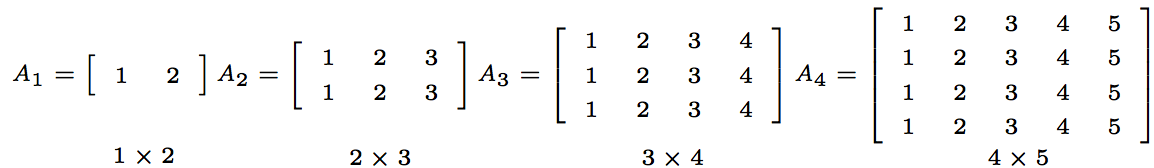
\includegraphics[width=5.4in] {L6-4matrices.png}
\end{figure}

\begin{eqnarray}
\text{\tt Solutions:} &    ( ( (A_1) (A_2) )  (A_3 ) )  ( A_4 )  &  (  ( A_1 )  (A_2 ) ) ( ( A_3 ) ( A_4 ) ) \nonumber \\
\text{\tt Cost:} &  1\times 2 \times 3  &  1  \times 2  \times 3   \nonumber \\
& +  1 \times 3 \times 4  & + 3 \times 4 \times 5 \nonumber  \\
& +  1 \times 4 \times 5  & + 1 \times 3 \times 5  \nonumber \\
& = 38 & =81 \nonumber
\end{eqnarray}

对这四个矩阵做运算,我们有很多种加括号的方案,比如:

方案一:先算$A_1*A_2$,然后再乘以$A_3$,最后乘以$A_4$,此时总共运算次数为38次。

方案二:先算$A_1*A_2$,然后算$A_3*A_4$,最后将两者得到的矩阵相乘,此时总的运算次数为81次。

我们使用两种不同的求解顺序,得到了不同的运算次数且差异很大。现在我们想知道第一种方案是最优的吗?是否存在更好的加括号的方案使得总共的运算次数最少。

\textbf{解空间:}

总共有多少种加括号的方案呢,实际上加括号的方案可以描述成一颗二叉树,二叉树的每个节点对应一个子问题。总共n个节点,则有${ 2n \choose n } - { 2n \choose n-1}$ (Catalan number ) 个从根节点到叶子节点的路径即${ 2n \choose n } - { 2n \choose n-1}$个加括号的方案。

卡特兰数是指数级别的,解空间非常大,如果暴力枚举的话,速度会非常慢,所以暴力枚举这种策略是不可行的。

\textbf{动态规划的一般思路:}

下面我们研究下动态规划是怎么进行求解的。

问题的求解还是基于我们的观察,现在给我们$n$个矩阵,我们不会做,我们可以看能不能把它分解成小问题来求解。

我们的解就是加括号的方案,把求解过程想象成一系列的决策。每一步的决策是确定在哪个位置加括号,即确定先算哪些矩阵,再算哪些矩阵。

假如当前我们拿到了一个最优解,我们记做 $O$ ,且假设我们将第一个括号加在第 $k$ 个矩阵与第 $k+1$ 个矩阵之间,即 ${(A_1 ... A_k)(A_{k+1}...A_{n})}$ ,也就是说我们要先算$(A_1 ... A_k)$,再算$(A_{k+1}...A_{n})$,最后将两部分得到的矩阵乘起来。

这样我们就把原始问题分解成在 $(A_1 ... A_k)$ 里面加括号使得运算次数最小和在 $(A_{k+1}...A_{n})$ 加括号使得运算次数最小两个子问题了。

我们可以发现左半部分的右下标需要改变,右半部分的左下标需要改变,因此该问题便是从$A_i$到$A_j$,这样问题的左右下标都可以变化。因此子问题一般形式表示为在 $(A_i,...,A_j)$ 加括号使得整体运算次数最少,我们记做 $OPT(i,j)$ , 显然原始问题可以表示成 $OPT(1,n)$.

因为左下标可以从$1$变化到$n$,而右下标可以从 $i$ 变化到$n$,因此原问题的解空间为$\sum_{i = 1}^n(n - i + 1) = \frac{n(n+1)}{2}$ ,即原问题包含 $O(n^2)$ 个子问题空间。

假如我们是在 $A_k$ 和 $A_{k+1}$ 矩阵之间加的括号,则在$A_i$到$A_j$所使用的运算次数就是

 \[Cost(i, j) = Cost(i, k) + Cost(k+1, j) + p_ip_{k+1}p_{j+1}\]

该表达式对于任意的解都有这个性质。因此我们考虑最优解这个特殊情况有:

\[OPT(i, j) = OPT(i, k) + OPT(k+1, j) + p_ip_{k+1}p_{j+1}\]

即 $(A_i,...,A_j)$ 最少的运算次数,等于$(A_i,...,A_k)$最少的运算次数加上$(A_k,...,A_j)$最少的运算次数加上最后两个矩阵相乘的运算次数。即原问题包含子问题的最优解,这就是最优子结构性质。

求解一个问题,如果这个问题可以规约,则分治大概可以解决问题。如果他还有最优子结构的性质,则动态规划大概可以解决问题。因此在碰到一个问题的时候,先观察该问题具有哪些性质,根据不同的性质我们使用不同的策略。

\subsection{最优子结构性质:}

那我们如何证明最优子结构呢:

如果对$(Ai,...,Ak)$有另外一种代价更小的加括号方案 $OPT‘(i,k) <OPT(i,k)$,那将它替换到 $(A_i,...A_j)$ 的最优加括号的策略中,就会产生另外一种加括号的方案,且代价小于最优代价 $OPT(i,j)$ ,这与原始定义$OPT(i,j)$ 是最优的矛盾。因此原问题一定包含子问题的最优解。

本问题隐含了独立性假设即左边的求解与右边的求解是彼此不影响的。

但是现在我们还不能知道k具体在哪个位置,因此需要在$i$和$j$区间内对$k$的所有情况进行枚举,则我们有如下递推表达式:

\begin{equation}
OPT(i, j) =
\begin{cases} 0 & i=j \\
{\bf min_{i\leq k < j} } \{OPT(i, k) + OPT(k+1, j) + p_ip_{k+1}p_{j+1} \} & otherwise
\end{cases} \nonumber
\end{equation}


现在我们可以利用得到的递归表达式,写出如下伪代码:
\\

%\begin{comment}

\begin{small}
{\sc RECURSIVE\_MATRIX\_CHAIN}$( i, j)$
\begin{algorithmic}[1]
\IF { $i == j$ }
\STATE return $0$;
\ENDIF
\STATE $OPT(i, j) = +\infty;$
\FOR{$k=i$ to $j-1$}
\STATE $q = $ {\sc RECURSIVE\_MATRIX\_CHAIN}$(i, k)$
\STATE $\quad  + $ {\sc RECURSIVE\_MATRIX\_CHAIN}$(k+1, j)$
\STATE $\quad  + p_ip_{k+1}p_{j+1} ;$
\IF { $q < OPT(i, j) $}
\STATE $OPT(i, j) = q;$
\ENDIF
\ENDFOR
\RETURN{ $OPT(i, j);$}
\end{algorithmic}
\end{small}
注意最优解可以通过调用 {\sc RECURSIVE\_MATRIX\_CHAIN}$(1, n)$ 得到.
\\
%\end{comment}

通过伪代码的递归形式,我们可以画出如下递归树:

\begin{figure}[htbp]
%\includegraphics[width=1.05\textwidth]{tree1.png}  %the original image
\begin{tikzpicture}[scale=0.8, auto,swap]
    % Draw a 7,11 network
    % First we draw the vertices
     \draw[thick] (0,0)  -- (4.5, -1);
     \draw[thick]  (0,0) --  (-4.5, -1);

     \draw[thick] (0,0)  -- (6.5, -1);
     \draw[thick]  (0,0) --  (-6.5, -1);
       \node[smallvertex,draw=black, fill=blue!20] (A4) at (6.5, -1) {};
        \node[smallvertex,draw=black, fill=blue!20] (A1) at (-6.5, -1) {};
   \node[left] at (A1.west) {\tiny $A_1$};
    \node[right] at (A4.east) {\tiny $A_{4}$};


    \def\dx{0};
    \def\dy{0}
    \foreach \pos/\name in {{(0+\dx,0+\dy)/R1}, {(-1+\dx,-1+\dy)/L}, {(1+\dx,-1+\dy)/R}, {(-1.5+\dx,-2+\dy)/LL}, {(-.5+\dx, -2+\dy)/LR}, {(0.5+\dx, -2+\dy)/RL}, {(1.5+\dx, -2+\dy)/RR}}
        \node[smallvertex,draw=black, fill=blue!20] (\name) at \pos {};
    % Connect vertices with edges and draw weights
    \foreach \source/ \dest /\weight in {R1/L/{}, R1/R/{}, L/LL/{}, L/LR/{}, R/RL/{}, R/RR/{}  }
        \path[undirectededge] (\source) -- node[weight] {$\weight$} (\dest);
%       \draw[dashed, ->] (0,0) arc  (120:60:2);
    \node[above] at (R1.north) {\tiny $A_1A_2A_3A_4$};
   \node[left] at (L.west) {\tiny $A_1A_2$};
   \node[right] at (R.east) {\tiny $A_3A_4$};
   \node[below] at (LL.south) {\tiny $A_1$};
   \node[below] at (LR.south) {\tiny $A_2$};
   \node[below] at (RL.south) {\tiny $A_3$};
    \node[below] at (RR.south) {\tiny $A_4$};




   %right sub-tree
      \draw[thick] (4.5,-1)  -- (2.5, -2);
      \draw[thick] (4.5,-1)  -- (6.5, -2);
       \node[smallvertex,draw=black, fill=blue!20] (A1) at (2.5,-2) {};
        \node[smallvertex,draw=black, fill=blue!20] (A3) at (6.5, -2) {};
  \node[below] at (A1.south) {\tiny $A_1$};
  \node[below] at (A3.south) {\tiny $A_3$};

    \def\dx{4.5};
    \def\dy{-1}
    \foreach \pos/\name in {{(0+\dx,0+\dy)/R1}, {(-1+\dx,-1+\dy)/L}, {(1+\dx,-1+\dy)/R}, {(-1.5+\dx,-2+\dy)/LL}, {(-.5+\dx, -2+\dy)/LR}, {(0.5+\dx, -2+\dy)/RL}, {(1.5+\dx, -2+\dy)/RR}}
        \node[smallvertex,draw=black, fill=blue!20] (\name) at \pos {};
    % Connect vertices with edges and draw weights
    \foreach \source/ \dest /\weight in {R1/L/{}, R1/R/{}, L/LL/{}, L/LR/{}, R/RL/{}, R/RR/{}  }
        \path[undirectededge] (\source) -- node[weight] {$\weight$} (\dest);
%       \draw[dashed, ->] (0,0) arc  (120:60:2);

    \node[left] at (R1.west) {\tiny $A_{1}A_2A_{3}$};
    \node[right] at (L) {\tiny $A_2A_{3}$};
    \node[left] at (R) {\tiny $A_1A_{2}$};
    \node[below] at (LL.south) {\tiny $A_2$};
    \node[below] at (LR.south) {\tiny $A_3$};
   \node[below] at (RL.south) {\tiny $A_1$};
   \node[below] at (RR.south) {\tiny $A_2$};




%left sub-tree

       \draw[thick] (-4.5,-1)  -- (-2.5, -2);
      \draw[thick] (-4.5,-1)  -- (-6.5, -2);
       \node[smallvertex,draw=black, fill=blue!20] (A2) at (-2.5,-2) {};
        \node[smallvertex,draw=black, fill=blue!20] (A4) at (-6.5, -2) {};
  \node[below] at (A2.south) {\tiny $A_4$};
  \node[below] at (A4.south) {\tiny $A_2$};


    \def\dx{-4.5};
    \def\dy{-1}
    \foreach \pos/\name in {{(0+\dx,0+\dy)/R1}, {(-1+\dx,-1+\dy)/L}, {(1+\dx,-1+\dy)/R}, {(-1.5+\dx,-2+\dy)/LL}, {(-.5+\dx, -2+\dy)/LR}, {(0.5+\dx, -2+\dy)/RL}, {(1.5+\dx, -2+\dy)/RR}}
        \node[smallvertex,draw=black, fill=blue!20] (\name) at \pos {};
    % Connect vertices with edges and draw weights
    \foreach \source/ \dest /\weight in {R1/L/{}, R1/R/{}, L/LL/{}, L/LR/{}, R/RL/{}, R/RR/{}  }
        \path[undirectededge] (\source) -- node[weight] {$\weight$} (\dest);
%       \draw[dashed, ->] (0,0) arc  (120:60:2);
      \node[right] at (R1.east) {\tiny $A_2A_{3}A_{4}$};
    \node[right] at (L) {\tiny $A_3A_{4}$};
    \node[left] at (R) {\tiny $A_2A_{3}$};
    \node[below] at (LL.south) {\tiny $A_3$};
    \node[below] at (LR.south) {\tiny $A_4$};
   \node[below] at (RL.south) {\tiny $A_2$};
   \node[below] at (RR.south) {\tiny $A_3$};




   \end{tikzpicture}
\end{figure}


递归树中的每个节点都代表一个子问题,我们可以发现上面的递归树中有很多节点是重复的。

\textbf{时间复杂度:}

现在我们求下该程序的时间复杂度:

假设$T(n)$ 为计算 $n$ 个矩阵乘积的复杂度,则有

$\qquad \qquad T(n) \geq 1 + \sum_{k=1}^{n-1} ( T(k) + T(n-k) + 1 )$ for $n > 1$

下面我们证明$T(n) \geq 2^{n-1}$,即原问题是指数时间的复杂度:

首先我们有$T(1) \geq 1 = 2^{1 - 1}$
然后针对$n > 1$ 的情况,我们有:
\begin{eqnarray}
T(n) & \geq &  1 + \sum\nolimits_{k=1}^{n-1} ( T(k) + T(n-k) + 1 ) \\
     & = & n + 2 \sum\nolimits_{k=1}^{n-1} T(k) \\
     & \geq & n + 2 \sum\nolimits_{k=1}^{n-1} 2^{k-1} \\
     & \geq & n + 2 ( 2^{n-1} - 1 ) \\
     & \geq & n + 2^n - 2 \\
     & \geq & 2^{n-1}
\end{eqnarray}

\subsection{记忆化搜索优化时间复杂度:}

现在有个问题,我们总共只有 $O(n^2)$ 个子问题,但是现在我们的程序竟然花费了 $2^n$ 时间,表明这里面肯定有子问题被重复计算了。

比如下图的红色节点:

\begin{figure}[htbp]
\centering
%\includegraphics[width=1.05\textwidth]{tree2.png}
\begin{tikzpicture}[scale=0.8, auto,swap]
    % Draw a 7,11 network
    % First we draw the vertices


     \draw[thick] (0,0)  -- (4.5, -1);
     \draw[thick]  (0,0) --  (-4.5, -1);

     \draw[thick] (0,0)  -- (6.5, -1);
     \draw[thick]  (0,0) --  (-6.5, -1);
       \node[smallvertex,draw=black, fill=red] (A4) at (6.5, -1) {};
        \node[smallvertex,draw=black, fill=blue!20] (A1) at (-6.5, -1) {};
   \node[left] at (A1.west) {\tiny $A_1$};
    \node[right] at (A4.east) {\tiny $A_{4}$};


%middle tree
    \def\dx{0};
    \def\dy{0}
    \foreach \pos/\name in {{(0+\dx,0+\dy)/R1}, {(-1+\dx,-1+\dy)/L}, {(1+\dx,-1+\dy)/R}, {(-1.5+\dx,-2+\dy)/LL}, {(-.5+\dx, -2+\dy)/LR}, {(0.5+\dx, -2+\dy)/RL}, {(1.5+\dx, -2+\dy)/RR}}
        \node[smallvertex,draw=black, fill=blue!20] (\name) at \pos {};
    % Connect vertices with edges and draw weights
    \foreach \source/ \dest /\weight in {R1/L/{}, R1/R/{}, L/LL/{}, L/LR/{}, R/RL/{}, R/RR/{}  }
        \path[undirectededge] (\source) -- node[weight] {$\weight$} (\dest);
%       \draw[dashed, ->] (0,0) arc  (120:60:2);
    \node[above] at (R1.north) {\tiny $A_1A_2A_3A_4$};
   \node[left] at (L.west) {\tiny $A_1A_2$};
   \node[right] at (R.east) {\tiny $A_3A_4$};
   \node[below] at (LL.south) {\tiny $A_1$};
   \node[below] at (LR.south) {\tiny $A_2$};
   \node[below] at (RL.south) {\tiny $A_3$};
    \node[below] at (RR.south) {\tiny $A_4$};

        \node[smallvertex,draw=black, fill=red]  at  (R) {};
        \node[smallvertex,draw=black, fill=red]  at  (LR) {};
         \node[smallvertex,draw=black, fill=red]  at  (RR) {};
                 \node[smallvertex,draw=black, fill=red]  at  (RL) {};



   %right sub-tree
      \draw[thick] (4.5,-1)  -- (2.5, -2);
      \draw[thick] (4.5,-1)  -- (6.5, -2);
       \node[smallvertex,draw=black, fill=red] (A1) at (2.5,-2) {};
        \node[smallvertex,draw=black, fill=red] (A3) at (6.5, -2) {};
  \node[below] at (A1.south) {\tiny $A_1$};
  \node[below] at (A3.south) {\tiny $A_3$};

    \def\dx{4.5};
    \def\dy{-1}
    \foreach \pos/\name in {{(0+\dx,0+\dy)/R1}, {(-1+\dx,-1+\dy)/L}, {(1+\dx,-1+\dy)/R}, {(-1.5+\dx,-2+\dy)/LL}, {(-.5+\dx, -2+\dy)/LR}, {(0.5+\dx, -2+\dy)/RL}, {(1.5+\dx, -2+\dy)/RR}}
        \node[smallvertex,draw=black, fill=blue!20] (\name) at \pos {};
    % Connect vertices with edges and draw weights
    \foreach \source/ \dest /\weight in {R1/L/{}, R1/R/{}, L/LL/{}, L/LR/{}, R/RL/{}, R/RR/{}  }
        \path[undirectededge] (\source) -- node[weight] {$\weight$} (\dest);
%       \draw[dashed, ->] (0,0) arc  (120:60:2);

    \node[left] at (R1.west) {\tiny $A_{1}A_2A_{3}$};
    \node[right] at (L) {\tiny $A_2A_{3}$};
    \node[left] at (R) {\tiny $A_1A_{2}$};
    \node[below] at (LL.south) {\tiny $A_2$};
    \node[below] at (LR.south) {\tiny $A_3$};
   \node[below] at (RL.south) {\tiny $A_1$};
   \node[below] at (RR.south) {\tiny $A_2$};

        \node[smallvertex,draw=black, fill=red]  at  (L) {};
        \node[smallvertex,draw=black, fill=red]  at  (R) {};
        \node[smallvertex,draw=black, fill=red]  at  (LR) {};
        \node[smallvertex,draw=black, fill=red]  at  (RR) {};
        \node[smallvertex,draw=black, fill=red]  at  (RL) {};
        \node[smallvertex,draw=black, fill=red]  at  (LL) {};




%left sub-tree

       \draw[thick] (-4.5,-1)  -- (-2.5, -2);
      \draw[thick] (-4.5,-1)  -- (-6.5, -2);
       \node[smallvertex,draw=black, fill=red] (A4) at (-2.5,-2) {};
        \node[smallvertex,draw=black, fill=blue!20] (A2) at (-6.5, -2) {};
  \node[below] at (A4.south) {\tiny $A_4$};
  \node[below] at (A2.south) {\tiny $A_2$};


    \def\dx{-4.5};
    \def\dy{-1}
    \foreach \pos/\name in {{(0+\dx,0+\dy)/R1}, {(-1+\dx,-1+\dy)/L}, {(1+\dx,-1+\dy)/R}, {(-1.5+\dx,-2+\dy)/LL}, {(-.5+\dx, -2+\dy)/LR}, {(0.5+\dx, -2+\dy)/RL}, {(1.5+\dx, -2+\dy)/RR}}
        \node[smallvertex,draw=black, fill=blue!20] (\name) at \pos {};
    % Connect vertices with edges and draw weights
    \foreach \source/ \dest /\weight in {R1/L/{}, R1/R/{}, L/LL/{}, L/LR/{}, R/RL/{}, R/RR/{}  }
        \path[undirectededge] (\source) -- node[weight] {$\weight$} (\dest);
%       \draw[dashed, ->] (0,0) arc  (120:60:2);
      \node[right] at (R1.east) {\tiny $A_2A_{3}A_{4}$};
    \node[right] at (L) {\tiny $A_3A_{4}$};
    \node[left] at (R) {\tiny $A_2A_{3}$};
    \node[below] at (LL.south) {\tiny $A_3$};
    \node[below] at (LR.south) {\tiny $A_4$};
   \node[below] at (RL.south) {\tiny $A_2$};
   \node[below] at (RR.south) {\tiny $A_3$};

        \node[smallvertex,draw=black, fill=red]  at  (RL) {};
         \node[smallvertex,draw=black, fill=red]  at  (RR) {};

   \end{tikzpicture}
\end{figure}


\newpage
我们直观的想法是可以将已经计算过的子问题保存在一张表里面。下次如果再求解该子问题则直接将表中存放的值返回即可,这样便避免了重复计算。

因此我们有下面伪代码:
\\
%\begin{comment}

\begin{small}
{\sc MEMORIZE\_MATRIX\_CHAIN}$( i, j)$
\begin{algorithmic}[1]
\IF{ \textcolor{red}{ $OPT[i, j] \neq NULL $ } }
\RETURN{ \textcolor{red}{ $OPT(i, j)$; } }
\ENDIF
\IF { $ i == j $ }
\STATE $OPT[ i, j] = 0;$
\ELSE
\FOR{$k= i$ to $j-1$}
\STATE $q = $   {\sc MEMORIZE\_MATRIX\_CHAIN}$(i, k)$
\STATE $\qquad  + ${\sc MEMORIZE\_MATRIX\_CHAIN}$( k+1, j)$
\STATE $\qquad  + p_ip_{k+1}p_{j+1} ;$
\IF { $q < OPT[i, j] $}
\STATE $OPT[i, j] = q;$
\ENDIF
\ENDFOR
\ENDIF
\RETURN{ $OPT[i, j];$ }
\end{algorithmic}
\end{small}

\indent

其实就是在原有伪代码的基础上添加了对表格中该单元的判断,如果该单元有值,则表明已经算过该子问题则直接返回,否则则对该子问题进行求解并保存在表格中。

因为原问题有 $O(n^2)$ 个子问题,每个子问题有 $O(n)$ 种选择,因此原问题的时间复杂度为O($n^3$)。

由于递归需要使用内存中的栈结构,运算速度稍微慢些,因此我们可以尝试使用非递归的形式自底向上进行计算。因此有以下伪代码:
\\

\begin{small}
{\sc MATRIX\_CHAIN\_MULTIPLICATION}$( P)$
\begin{algorithmic}[1]
\FOR {$i=1$ to $n$ }
\STATE $OPT(i,i)=0;$
\ENDFOR
\FOR {$l=2$ to $n$ }
  \FOR {$i=1$ to $n-l+1$ }
    \STATE $j=i+l-1;$
    \STATE $OPT(i,j)=+\infty$;
    \FOR{$k= i$ to $j-1$}
      \STATE $q = OPT(i,k) + OPT(k+1,j) +  p_ip_{k+1}p_{j+1} ;$
      \IF { $q < OPT(i, j) $}
	\STATE $OPT(i, j) = q;$
	\STATE $S(i,j) = k;$
      \ENDIF
    \ENDFOR
  \ENDFOR
\ENDFOR
\RETURN{ $OPT(1,n)$;}
\end{algorithmic}
\end{small}

\indent

因此我们有以下的运算过程:

\begin{figure}[htbp]
%\includegraphics[width=1.05\textwidth]{tree3.png}
\begin{tikzpicture}[scale=0.8, auto,swap]
    % Draw a 7,11 network
    % First we draw the vertices


     \draw[thick] (0,0)  -- (4.5, -1);
     \draw[thick]  (0,0) --  (-4.5, -1);

     \draw[thick] (0,0)  -- (6.5, -1);
     \draw[thick]  (0,0) --  (-6.5, -1);
       \node[smallvertex,draw=black, fill=red] (A4) at (6.5, -1) {};
        \node[smallvertex,draw=black, fill=red] (A1) at (-6.5, -1) {};
   \node[left] at (A1.west) {\tiny $A_1$};
    \node[right] at (A4.east) {\tiny $A_{4}$};


%middle tree
    \def\dx{0};
    \def\dy{0}
    \foreach \pos/\name in {{(0+\dx,0+\dy)/R1}, {(-1+\dx,-1+\dy)/L}, {(1+\dx,-1+\dy)/R}, {(-1.5+\dx,-2+\dy)/LL}, {(-.5+\dx, -2+\dy)/LR}, {(0.5+\dx, -2+\dy)/RL}, {(1.5+\dx, -2+\dy)/RR}}
        \node[smallvertex,draw=black, fill=blue!20] (\name) at \pos {};
    % Connect vertices with edges and draw weights
    \foreach \source/ \dest /\weight in {R1/L/{}, R1/R/{}, L/LL/{}, L/LR/{}, R/RL/{}, R/RR/{}  }
        \path[undirectededge] (\source) -- node[weight] {$\weight$} (\dest);
%       \draw[dashed, ->] (0,0) arc  (120:60:2);
    \node[above] at (R1.north) {\tiny $A_1A_2A_3A_4$};
   \node[left] at (L.west) {\tiny $A_1A_2$};
   \node[right] at (R.east) {\tiny $A_3A_4$};
   \node[below] at (LL.south) {\tiny $A_1$};
   \node[below] at (LR.south) {\tiny $A_2$};
   \node[below] at (RL.south) {\tiny $A_3$};
    \node[below] at (RR.south) {\tiny $A_4$};

  \node[smallvertex,draw=black, fill=blue]  at  (R1) {};
  \node[smallvertex,draw=black, fill=green]  at  (L) {};
  \node[smallvertex,draw=black, fill=green]  at  (R) {};
        \node[smallvertex,draw=black, fill=red]  at  (LL) {};
        \node[smallvertex,draw=black, fill=red]  at  (LR) {};
         \node[smallvertex,draw=black, fill=red]  at  (RR) {};
                 \node[smallvertex,draw=black, fill=red]  at  (RL) {};



   %right sub-tree
      \draw[thick] (4.5,-1)  -- (2.5, -2);
      \draw[thick] (4.5,-1)  -- (6.5, -2);
       \node[smallvertex,draw=black, fill=red] (A1) at (2.5,-2) {};
        \node[smallvertex,draw=black, fill=red] (A3) at (6.5, -2) {};
  \node[below] at (A1.south) {\tiny $A_1$};
  \node[below] at (A3.south) {\tiny $A_3$};

    \def\dx{4.5};
    \def\dy{-1}
    \foreach \pos/\name in {{(0+\dx,0+\dy)/R1}, {(-1+\dx,-1+\dy)/L}, {(1+\dx,-1+\dy)/R}, {(-1.5+\dx,-2+\dy)/LL}, {(-.5+\dx, -2+\dy)/LR}, {(0.5+\dx, -2+\dy)/RL}, {(1.5+\dx, -2+\dy)/RR}}
        \node[smallvertex,draw=black, fill=blue!20] (\name) at \pos {};
    % Connect vertices with edges and draw weights
    \foreach \source/ \dest /\weight in {R1/L/{}, R1/R/{}, L/LL/{}, L/LR/{}, R/RL/{}, R/RR/{}  }
        \path[undirectededge] (\source) -- node[weight] {$\weight$} (\dest);
%       \draw[dashed, ->] (0,0) arc  (120:60:2);

    \node[left] at (R1.west) {\tiny $A_{1}A_2A_{3}$};
    \node[right] at (L) {\tiny $A_2A_{3}$};
    \node[left] at (R) {\tiny $A_1A_{2}$};
    \node[below] at (LL.south) {\tiny $A_2$};
    \node[below] at (LR.south) {\tiny $A_3$};
   \node[below] at (RL.south) {\tiny $A_1$};
   \node[below] at (RR.south) {\tiny $A_2$};

        \node[smallvertex,draw=black, fill=orange]  at  (R1) {};
        \node[smallvertex,draw=black, fill=green]  at  (L) {};
        \node[smallvertex,draw=black, fill=green]  at  (R) {};
        \node[smallvertex,draw=black, fill=red]  at  (LR) {};
        \node[smallvertex,draw=black, fill=red]  at  (RR) {};
        \node[smallvertex,draw=black, fill=red]  at  (RL) {};
        \node[smallvertex,draw=black, fill=red]  at  (LL) {};




%left sub-tree

       \draw[thick] (-4.5,-1)  -- (-2.5, -2);
      \draw[thick] (-4.5,-1)  -- (-6.5, -2);
       \node[smallvertex,draw=black, fill=red] (A4) at (-2.5,-2) {};
        \node[smallvertex,draw=black, fill=red] (A2) at (-6.5, -2) {};
  \node[below] at (A4.south) {\tiny $A_4$};
  \node[below] at (A2.south) {\tiny $A_2$};


    \def\dx{-4.5};
    \def\dy{-1}
    \foreach \pos/\name in {{(0+\dx,0+\dy)/R1}, {(-1+\dx,-1+\dy)/L}, {(1+\dx,-1+\dy)/R}, {(-1.5+\dx,-2+\dy)/LL}, {(-.5+\dx, -2+\dy)/LR}, {(0.5+\dx, -2+\dy)/RL}, {(1.5+\dx, -2+\dy)/RR}}
        \node[smallvertex,draw=black, fill=blue!20] (\name) at \pos {};
    % Connect vertices with edges and draw weights
    \foreach \source/ \dest /\weight in {R1/L/{}, R1/R/{}, L/LL/{}, L/LR/{}, R/RL/{}, R/RR/{}  }
        \path[undirectededge] (\source) -- node[weight] {$\weight$} (\dest);
%       \draw[dashed, ->] (0,0) arc  (120:60:2);
      \node[right] at (R1.east) {\tiny $A_2A_{3}A_{4}$};
    \node[right] at (L) {\tiny $A_3A_{4}$};
    \node[left] at (R) {\tiny $A_2A_{3}$};
    \node[below] at (LL.south) {\tiny $A_3$};
    \node[below] at (LR.south) {\tiny $A_4$};
   \node[below] at (RL.south) {\tiny $A_2$};
   \node[below] at (RR.south) {\tiny $A_3$};


        \node[smallvertex,draw=black, fill=orange]  at  (R1) {};
        \node[smallvertex,draw=black, fill=green]  at  (L) {};
        \node[smallvertex,draw=black, fill=green]  at  (R) {};
        \node[smallvertex,draw=black, fill=red]  at  (LR) {};
        \node[smallvertex,draw=black, fill=red]  at  (RR) {};
        \node[smallvertex,draw=black, fill=red]  at  (RL) {};
        \node[smallvertex,draw=black, fill=red]  at  (LL) {};



   \end{tikzpicture}
\end{figure}

(1)求解红色(叶子)节点上的子问题。

(2)求解绿色节点上的子问题。

(3)求解橘黄色节点上的子问题。

(4)得到原问题的最优解。

我们可以看到动态规划是自低向上求解最优解问题的。

\indent
\subsection{具体事例运算过程:}

下面我们详细看下动态规划求解矩阵链式乘法的运算过程:

\begin{figure}[htbp]
\centering
%\includegraphics[width=0.55\textwidth]{tree4.png}
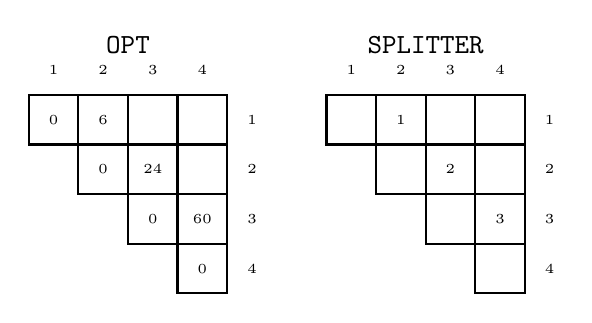
\begin{tikzpicture}[scale=0.9, auto,swap]

  	\def\d{0.7};
	
	%draw index
 \def\dy{1};
 \def\dx{0};
 \node at ( 2 * \d + \dx * \d, \dy * \d +  \d ) {\tt OPT };

    \foreach \i/\num/\name in { 1/1/s1,2/2/s2,3/3/s3,4/4/s4 }{
           \node (\name) at (\i*\d+\d/2 + \dx*\d - \d, \d/2 + \dy * \d) {\tiny $\num$};
    }

 \def\dy{0};
 \def\dx{0};
    \foreach \i/\num/\name in { 1/1/s1,2/2/s2,3/3/s3,4/4/s4 }{
         \node (\name) at ( 4*\d+\d/2  + \dx * \d,  0.0 - \i*\d + \d/2 - \dy * \d + \d){\tiny $\num$};
    }


	
 \def\dy{0};
 \def\dx{0};
    \foreach \i/\num/\name in { 0/0/s8,1/6/s7,2//s6,3//s5 }{
             \draw[  thick ] (\i*\d + \dx*\d,  0+ \dy*\d) rectangle (\i*\d+\d + \dx*\d, \d + \dy*\d);
         \node (\name) at (\i*\d+\d/2 + \dx*\d, \d/2 + \dy*\d) {\tiny $\num$};
    }
 \def\dy{-1};
 \def\dx{1};
    \foreach \i/\num/\name in { 0/0/s8,1/24/s7,2//s6}{
             \draw[  thick ] (\i*\d + \dx*\d,  0+ \dy*\d) rectangle (\i*\d+\d + \dx*\d, \d + \dy*\d);
         \node (\name) at (\i*\d+\d/2 + \dx*\d, \d/2 + \dy*\d) {\tiny $\num$};
    }
 \def\dy{-2};
 \def\dx{2};
    \foreach \i/\num/\name in { 0/0/s8,1/60/s7}{
             \draw[  thick ] (\i*\d + \dx*\d,  0+ \dy*\d) rectangle (\i*\d+\d + \dx*\d, \d + \dy*\d);
         \node (\name) at (\i*\d+\d/2 + \dx*\d, \d/2 + \dy*\d) {\tiny $\num$};
    }
     \def\dy{-3};
 \def\dx{3};
    \foreach \i/\num/\name in { 0/0/s8}{
             \draw[  thick ] (\i*\d + \dx*\d,  0+ \dy*\d) rectangle (\i*\d+\d + \dx*\d, \d + \dy*\d);
         \node (\name) at (\i*\d+\d/2 + \dx*\d, \d/2 + \dy*\d) {\tiny $\num$};
    }










   %split
   	%draw index
 \def\dy{1};
 \def\dx{6};
 \node at ( 2 * \d + \dx * \d, \dy * \d +  \d ) {\tt SPLITTER};

    \foreach \i/\num/\name in { 1/1/s1,2/2/s2,3/3/s3,4/4/s4 }{
           \node (\name) at (\i*\d+\d/2 + \dx*\d - \d, \d/2 + \dy * \d) {\tiny $\num$};
    }

 \def\dy{0};
 \def\dx{6};
    \foreach \i/\num/\name in { 1/1/s1,2/2/s2,3/3/s3,4/4/s4 }{
         \node (\name) at ( 4*\d+\d/2  + \dx * \d,  0.0 - \i*\d + \d/2 - \dy * \d + \d){\tiny $\num$};
    }


	
 \def\dy{0};
 \def\dx{6};
    \foreach \i/\num/\name in { 0//s8,1/1/s7,2//s6,3//s5 }{
             \draw[  thick ] (\i*\d + \dx*\d,  0+ \dy*\d) rectangle (\i*\d+\d + \dx*\d, \d + \dy*\d);
         \node (\name) at (\i*\d+\d/2 + \dx*\d, \d/2 + \dy*\d) {\tiny $\num$};
    }
 \def\dy{-1};
 \def\dx{7};
    \foreach \i/\num/\name in { 0//s8,1/2/s7,2//s6}{
             \draw[  thick ] (\i*\d + \dx*\d,  0+ \dy*\d) rectangle (\i*\d+\d + \dx*\d, \d + \dy*\d);
         \node (\name) at (\i*\d+\d/2 + \dx*\d, \d/2 + \dy*\d) {\tiny $\num$};
    }
 \def\dy{-2};
 \def\dx{8};
    \foreach \i/\num/\name in { 0//s8,1/3/s7}{
             \draw[  thick ] (\i*\d + \dx*\d,  0+ \dy*\d) rectangle (\i*\d+\d + \dx*\d, \d + \dy*\d);
         \node (\name) at (\i*\d+\d/2 + \dx*\d, \d/2 + \dy*\d) {\tiny $\num$};
    }
     \def\dy{-3};
 \def\dx{9};
    \foreach \i/\num/\name in { 0//s8}{
             \draw[  thick ] (\i*\d + \dx*\d,  0+ \dy*\d) rectangle (\i*\d+\d + \dx*\d, \d + \dy*\d);
         \node (\name) at (\i*\d+\d/2 + \dx*\d, \d/2 + \dy*\d) {\tiny $\num$};
    }




\end{tikzpicture}

\begin{flushleft}
第一步:

$OPT[1,2] = p_{0} \times p_{1} \times p_{2}  = 1\times 2 \times 3 = 6; $

$OPT[2,3] = p_{1} \times p_{2} \times p_{3}  = 2\times 3 \times 4 = 24; $

$OPT[3,4] = p_{2} \times p_{3} \times p_{4}  = 3\times 4 \times 5 = 60; $
\end{flushleft}

\end{figure}

\newpage
\begin{figure}[htbp]
\centering
%\includegraphics[width=0.55\textwidth]{tree5.png}
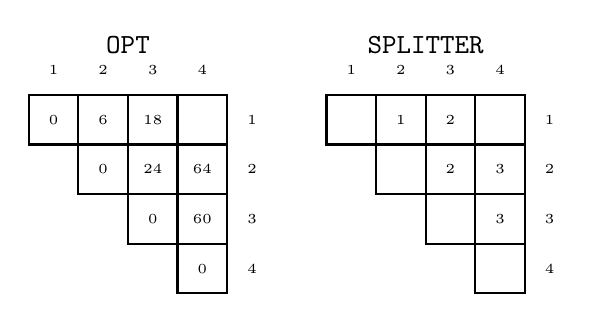
\begin{tikzpicture}[scale=0.9, auto,swap]

  	\def\d{0.7};
	
	%draw index
 \def\dy{1};
 \def\dx{0};
 \node at ( 2 * \d + \dx * \d, \dy * \d +  \d ) {\tt OPT };

    \foreach \i/\num/\name in { 1/1/s1,2/2/s2,3/3/s3,4/4/s4 }{
           \node (\name) at (\i*\d+\d/2 + \dx*\d - \d, \d/2 + \dy * \d) {\tiny $\num$};
    }

 \def\dy{0};
 \def\dx{0};
    \foreach \i/\num/\name in { 1/1/s1,2/2/s2,3/3/s3,4/4/s4 }{
         \node (\name) at ( 4*\d+\d/2  + \dx * \d,  0.0 - \i*\d + \d/2 - \dy * \d + \d){\tiny $\num$};
    }


	
 \def\dy{0};
 \def\dx{0};
    \foreach \i/\num/\name in { 0/0/s8,1/6/s7,2/18/s6,3//s5 }{
             \draw[  thick ] (\i*\d + \dx*\d,  0+ \dy*\d) rectangle (\i*\d+\d + \dx*\d, \d + \dy*\d);
         \node (\name) at (\i*\d+\d/2 + \dx*\d, \d/2 + \dy*\d) {\tiny $\num$};
    }
 \def\dy{-1};
 \def\dx{1};
    \foreach \i/\num/\name in { 0/0/s8,1/24/s7,2/64/s6}{
             \draw[  thick ] (\i*\d + \dx*\d,  0+ \dy*\d) rectangle (\i*\d+\d + \dx*\d, \d + \dy*\d);
         \node (\name) at (\i*\d+\d/2 + \dx*\d, \d/2 + \dy*\d) {\tiny $\num$};
    }
 \def\dy{-2};
 \def\dx{2};
    \foreach \i/\num/\name in { 0/0/s8,1/60/s7}{
             \draw[  thick ] (\i*\d + \dx*\d,  0+ \dy*\d) rectangle (\i*\d+\d + \dx*\d, \d + \dy*\d);
         \node (\name) at (\i*\d+\d/2 + \dx*\d, \d/2 + \dy*\d) {\tiny $\num$};
    }
     \def\dy{-3};
 \def\dx{3};
    \foreach \i/\num/\name in { 0/0/s8}{
             \draw[  thick ] (\i*\d + \dx*\d,  0+ \dy*\d) rectangle (\i*\d+\d + \dx*\d, \d + \dy*\d);
         \node (\name) at (\i*\d+\d/2 + \dx*\d, \d/2 + \dy*\d) {\tiny $\num$};
    }










   %split
   	%draw index
 \def\dy{1};
 \def\dx{6};
 \node at ( 2 * \d + \dx * \d, \dy * \d +  \d ) {\tt SPLITTER};

    \foreach \i/\num/\name in { 1/1/s1,2/2/s2,3/3/s3,4/4/s4 }{
           \node (\name) at (\i*\d+\d/2 + \dx*\d - \d, \d/2 + \dy * \d) {\tiny $\num$};
    }

 \def\dy{0};
 \def\dx{6};
    \foreach \i/\num/\name in { 1/1/s1,2/2/s2,3/3/s3,4/4/s4 }{
         \node (\name) at ( 4*\d+\d/2  + \dx * \d,  0.0 - \i*\d + \d/2 - \dy * \d + \d){\tiny $\num$};
    }


	
 \def\dy{0};
 \def\dx{6};
    \foreach \i/\num/\name in { 0//s8,1/1/s7,2/2/s6,3//s5 }{
             \draw[  thick ] (\i*\d + \dx*\d,  0+ \dy*\d) rectangle (\i*\d+\d + \dx*\d, \d + \dy*\d);
         \node (\name) at (\i*\d+\d/2 + \dx*\d, \d/2 + \dy*\d) {\tiny $\num$};
    }
 \def\dy{-1};
 \def\dx{7};
    \foreach \i/\num/\name in { 0//s8,1/2/s7,2/3/s6}{
             \draw[  thick ] (\i*\d + \dx*\d,  0+ \dy*\d) rectangle (\i*\d+\d + \dx*\d, \d + \dy*\d);
         \node (\name) at (\i*\d+\d/2 + \dx*\d, \d/2 + \dy*\d) {\tiny $\num$};
    }
 \def\dy{-2};
 \def\dx{8};
    \foreach \i/\num/\name in { 0//s8,1/3/s7}{
             \draw[  thick ] (\i*\d + \dx*\d,  0+ \dy*\d) rectangle (\i*\d+\d + \dx*\d, \d + \dy*\d);
         \node (\name) at (\i*\d+\d/2 + \dx*\d, \d/2 + \dy*\d) {\tiny $\num$};
    }
     \def\dy{-3};
 \def\dx{9};
    \foreach \i/\num/\name in { 0//s8}{
             \draw[  thick ] (\i*\d + \dx*\d,  0+ \dy*\d) rectangle (\i*\d+\d + \dx*\d, \d + \dy*\d);
         \node (\name) at (\i*\d+\d/2 + \dx*\d, \d/2 + \dy*\d) {\tiny $\num$};
    }




\end{tikzpicture}
\begin{flushleft}
第二步:

\begin{small}
$OPT[1,3] = \min \begin{cases} OPT[1,2] + OPT[3,3] + p_{0} \times p_{3} \times p_{4}  (=18) \\
OPT[1,1] + OPT[2,3] + p_{0} \times p_{2} \times p_{4}  (=32)
\end{cases}$
Thus, $SPLITTER[1,2] =2$.  \ \\
\ \\

$OPT[2,4] = \min \begin{cases} OPT[2,2] + OPT[3,4] + p_{1} \times p_{2} \times p_{4}  (=90) \\
OPT[2,3] + OPT[4,4] + p_{1} \times p_{3} \times p_{4}  (=64)
\end{cases}$
Thus, $SPLITTER[2,4] =3$.

\end{small}
\end{flushleft}

\end{figure}



\begin{figure}[htbp]
\centering
%\includegraphics[width=0.55\textwidth]{tree6.png}
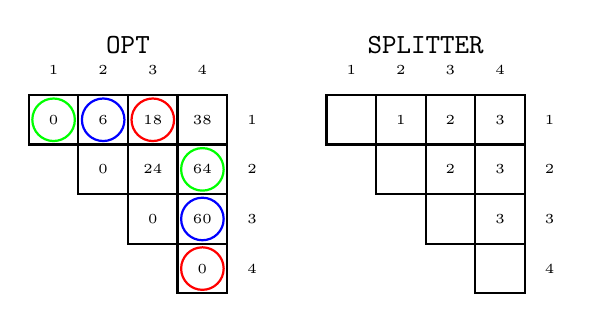
\begin{tikzpicture}[scale=0.9, auto,swap]

  	\def\d{0.7};
	
	%draw index
 \def\dy{1};
 \def\dx{0};
 \node at ( 2 * \d + \dx * \d, \dy * \d +  \d ) {\tt OPT };

    \foreach \i/\num/\name in { 1/1/s1,2/2/s2,3/3/s3,4/4/s4 }{
           \node (\name) at (\i*\d+\d/2 + \dx*\d - \d, \d/2 + \dy * \d) {\tiny $\num$};
    }

 \def\dy{0};
 \def\dx{0};
    \foreach \i/\num/\name in { 1/1/s1,2/2/s2,3/3/s3,4/4/s4 }{
         \node (\name) at ( 4*\d+\d/2  + \dx * \d,  0.0 - \i*\d + \d/2 - \dy * \d + \d){\tiny $\num$};
    }


	
 \def\dy{0};
 \def\dx{0};
    \foreach \i/\num/\name in { 0/0/s8,1/6/s7,2/18/s6,3/38/s5 }{
             \draw[  thick ] (\i*\d + \dx*\d,  0+ \dy*\d) rectangle (\i*\d+\d + \dx*\d, \d + \dy*\d);
         \node (\name) at (\i*\d+\d/2 + \dx*\d, \d/2 + \dy*\d) {\tiny $\num$};
    }
      \draw[thick, green] (s8) circle [radius=0.3];
      \draw[thick, blue] (s7) circle [radius=0.3];
            \draw[thick, red] (s6) circle [radius=0.3];

 \def\dy{-1};
 \def\dx{1};
    \foreach \i/\num/\name in { 0/0/s8,1/24/s7,2/64/s6}{
             \draw[  thick ] (\i*\d + \dx*\d,  0+ \dy*\d) rectangle (\i*\d+\d + \dx*\d, \d + \dy*\d);
         \node (\name) at (\i*\d+\d/2 + \dx*\d, \d/2 + \dy*\d) {\tiny $\num$};
    }
          \draw[thick, green] (s6) circle [radius=0.3];

 \def\dy{-2};
 \def\dx{2};
    \foreach \i/\num/\name in { 0/0/s8,1/60/s7}{
             \draw[  thick ] (\i*\d + \dx*\d,  0+ \dy*\d) rectangle (\i*\d+\d + \dx*\d, \d + \dy*\d);
         \node (\name) at (\i*\d+\d/2 + \dx*\d, \d/2 + \dy*\d) {\tiny $\num$};
    }
              \draw[thick, blue] (s7) circle [radius=0.3];

     \def\dy{-3};
 \def\dx{3};
    \foreach \i/\num/\name in { 0/0/s8}{
             \draw[  thick ] (\i*\d + \dx*\d,  0+ \dy*\d) rectangle (\i*\d+\d + \dx*\d, \d + \dy*\d);
         \node (\name) at (\i*\d+\d/2 + \dx*\d, \d/2 + \dy*\d) {\tiny $\num$};
    }
              \draw[thick, red] (s8) circle [radius=0.3];









   %split
   	%draw index
 \def\dy{1};
 \def\dx{6};
 \node at ( 2 * \d + \dx * \d, \dy * \d +  \d ) {\tt SPLITTER};

    \foreach \i/\num/\name in { 1/1/s1,2/2/s2,3/3/s3,4/4/s4 }{
           \node (\name) at (\i*\d+\d/2 + \dx*\d - \d, \d/2 + \dy * \d) {\tiny $\num$};
    }

 \def\dy{0};
 \def\dx{6};
    \foreach \i/\num/\name in { 1/1/s1,2/2/s2,3/3/s3,4/4/s4 }{
         \node (\name) at ( 4*\d+\d/2  + \dx * \d,  0.0 - \i*\d + \d/2 - \dy * \d + \d){\tiny $\num$};
    }


	
 \def\dy{0};
 \def\dx{6};
    \foreach \i/\num/\name in { 0//s8,1/1/s7,2/2/s6,3/3/s5 }{
             \draw[  thick ] (\i*\d + \dx*\d,  0+ \dy*\d) rectangle (\i*\d+\d + \dx*\d, \d + \dy*\d);
         \node (\name) at (\i*\d+\d/2 + \dx*\d, \d/2 + \dy*\d) {\tiny $\num$};
    }


 \def\dy{-1};
 \def\dx{7};
    \foreach \i/\num/\name in { 0//s8,1/2/s7,2/3/s6}{
             \draw[  thick ] (\i*\d + \dx*\d,  0+ \dy*\d) rectangle (\i*\d+\d + \dx*\d, \d + \dy*\d);
         \node (\name) at (\i*\d+\d/2 + \dx*\d, \d/2 + \dy*\d) {\tiny $\num$};
    }
 \def\dy{-2};
 \def\dx{8};
    \foreach \i/\num/\name in { 0//s8,1/3/s7}{
             \draw[  thick ] (\i*\d + \dx*\d,  0+ \dy*\d) rectangle (\i*\d+\d + \dx*\d, \d + \dy*\d);
         \node (\name) at (\i*\d+\d/2 + \dx*\d, \d/2 + \dy*\d) {\tiny $\num$};
    }
     \def\dy{-3};
 \def\dx{9};
    \foreach \i/\num/\name in { 0//s8}{
             \draw[  thick ] (\i*\d + \dx*\d,  0+ \dy*\d) rectangle (\i*\d+\d + \dx*\d, \d + \dy*\d);
         \node (\name) at (\i*\d+\d/2 + \dx*\d, \d/2 + \dy*\d) {\tiny $\num$};
    }




\end{tikzpicture}
\begin{flushleft}
第三步:

\begin{small}
$OPT[1,4] = \min \begin{cases} OPT[1,1] + OPT[2,4] + p_{0} \times p_{1} \times p_{4}  (=74) \\
OPT[1,2] + OPT[3,4] + p_{0} \times p_{2} \times p_{4}  (=81)  \\
OPT[1,3] + OPT[4,4] + p_{0} \times p_{3} \times p_{4}  (=38)
\end{cases}$
Thus, $SPLITTER[1,4] = 3$.
\end{small}
\end{flushleft}
\end{figure}


\newpage

经过我们一步步的计算最后得到结果是 $38$ ,即我们运用动态规划得到的第一种方案是最好的方案。

\subsection{构建最优解方案:}

虽然我们找到了最优解的值,但是怎样求得与该最优解对应的解方案呢。

我们的解决方案是进行回溯,需要我们另外使用一个数组S保存当前节点最优解的来源。比如$S[i,j]$ 是记录 了对乘积$A_i,...,A_j$ 在$A_k$ 与$A_{k + 1}$ 之间进行分开以取得最优加括号方案的 $k$ 值。

因此原问题$A_1,...,A_n$的最优解方案就是$(A_1,...,A_{S[1,n]})(A_{S[1,n] + 1},...,A_n)$ .

这里我们需要注意:原问题的最优解只有当所有的子问题都被算出来后才能得到。

下面我们尝试回溯找到最优解方案:

\begin{figure}[htbp]
\centering
%\includegraphics[width=0.55\textwidth]{tree7.png}
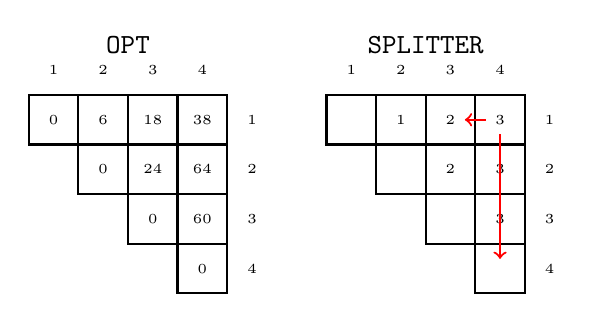
\begin{tikzpicture}[scale=0.9, auto,swap]

  	\def\d{0.7};


   	\def\d{0.7};
	
	%draw index
 \def\dy{1};
 \def\dx{0};
 \node at ( 2 * \d + \dx * \d, \dy * \d +  \d ) {\tt OPT };

    \foreach \i/\num/\name in { 1/1/s1,2/2/s2,3/3/s3,4/4/s4 }{
           \node (\name) at (\i*\d+\d/2 + \dx*\d - \d, \d/2 + \dy * \d) {\tiny $\num$};
    }

 \def\dy{0};
 \def\dx{0};
    \foreach \i/\num/\name in { 1/1/s1,2/2/s2,3/3/s3,4/4/s4 }{
         \node (\name) at ( 4*\d+\d/2  + \dx * \d,  0.0 - \i*\d + \d/2 - \dy * \d + \d){\tiny $\num$};
    }


	
 \def\dy{0};
 \def\dx{0};
    \foreach \i/\num/\name in { 0/0/s8,1/6/s7,2/18/s6,3/38/s5 }{
             \draw[  thick ] (\i*\d + \dx*\d,  0+ \dy*\d) rectangle (\i*\d+\d + \dx*\d, \d + \dy*\d);
         \node (\name) at (\i*\d+\d/2 + \dx*\d, \d/2 + \dy*\d) {\tiny $\num$};
    }
%      \draw[thick, green] (s8) circle [radius=0.3];
%      \draw[thick, blue] (s7) circle [radius=0.3];
%            \draw[thick, red] (s6) circle [radius=0.3];

 \def\dy{-1};
 \def\dx{1};
    \foreach \i/\num/\name in { 0/0/s8,1/24/s7,2/64/s6}{
             \draw[  thick ] (\i*\d + \dx*\d,  0+ \dy*\d) rectangle (\i*\d+\d + \dx*\d, \d + \dy*\d);
         \node (\name) at (\i*\d+\d/2 + \dx*\d, \d/2 + \dy*\d) {\tiny $\num$};
    }
        %  \draw[thick, green] (s6) circle [radius=0.3];

 \def\dy{-2};
 \def\dx{2};
    \foreach \i/\num/\name in { 0/0/s8,1/60/s7}{
             \draw[  thick ] (\i*\d + \dx*\d,  0+ \dy*\d) rectangle (\i*\d+\d + \dx*\d, \d + \dy*\d);
         \node (\name) at (\i*\d+\d/2 + \dx*\d, \d/2 + \dy*\d) {\tiny $\num$};
    }
            %  \draw[thick, blue] (s7) circle [radius=0.3];

     \def\dy{-3};
 \def\dx{3};
    \foreach \i/\num/\name in { 0/0/s8}{
             \draw[  thick ] (\i*\d + \dx*\d,  0+ \dy*\d) rectangle (\i*\d+\d + \dx*\d, \d + \dy*\d);
         \node (\name) at (\i*\d+\d/2 + \dx*\d, \d/2 + \dy*\d) {\tiny $\num$};
    }
         %     \draw[thick, red] (s8) circle [radius=0.3];


   %split
   	%draw index
 \def\dy{1};
 \def\dx{6};
 \node at ( 2 * \d + \dx * \d, \dy * \d +  \d ) {\tt SPLITTER};

    \foreach \i/\num/\name in { 1/1/s1,2/2/s2,3/3/s3,4/4/s4 }{
           \node (\name) at (\i*\d+\d/2 + \dx*\d - \d, \d/2 + \dy * \d) {\tiny $\num$};
    }

 \def\dy{0};
 \def\dx{6};
    \foreach \i/\num/\name in { 1/1/s1,2/2/s2,3/3/s3,4/4/s4 }{
         \node (\name) at ( 4*\d+\d/2  + \dx * \d,  0.0 - \i*\d + \d/2 - \dy * \d + \d){\tiny $\num$};
    }


	
 \def\dy{0};
 \def\dx{6};
    \foreach \i/\num/\name in { 0//s11,1/1/s12,2/2/s13,3/3/s14}{
             \draw[  thick ] (\i*\d + \dx*\d,  0+ \dy*\d) rectangle (\i*\d+\d + \dx*\d, \d + \dy*\d);
         \node (\name) at (\i*\d+\d/2 + \dx*\d, \d/2 + \dy*\d) {\tiny $\num$};
    }


 \def\dy{-1};
 \def\dx{7};
    \foreach \i/\num/\name in { 0//s21,1/2/s22,2/3/s23}{
             \draw[  thick ] (\i*\d + \dx*\d,  0+ \dy*\d) rectangle (\i*\d+\d + \dx*\d, \d + \dy*\d);
         \node (\name) at (\i*\d+\d/2 + \dx*\d, \d/2 + \dy*\d) {\tiny $\num$};
    }
 \def\dy{-2};
 \def\dx{8};
    \foreach \i/\num/\name in { 0//s31,1/3/s32}{
             \draw[  thick ] (\i*\d + \dx*\d,  0+ \dy*\d) rectangle (\i*\d+\d + \dx*\d, \d + \dy*\d);
         \node (\name) at (\i*\d+\d/2 + \dx*\d, \d/2 + \dy*\d) {\tiny $\num$};
    }
     \def\dy{-3};
 \def\dx{9};
    \foreach \i/\num/\name in { 0//s41}{
             \draw[  thick ] (\i*\d + \dx*\d,  0+ \dy*\d) rectangle (\i*\d+\d + \dx*\d, \d + \dy*\d);
         \node (\name) at (\i*\d+\d/2 + \dx*\d, \d/2 + \dy*\d) {\tiny $\num$};
    }

\draw[red, thick, ->] (s14) -- (s13);
\draw[red, thick, ->] (s14) -- (s41);

\end{tikzpicture}
\begin{flushleft}
第一步:    $(A_1A_2A_3)(A_4)$
\end{flushleft}
\end{figure}



\begin{figure}[htbp]
\centering
%\includegraphics[width=0.55\textwidth]{tree8.png}
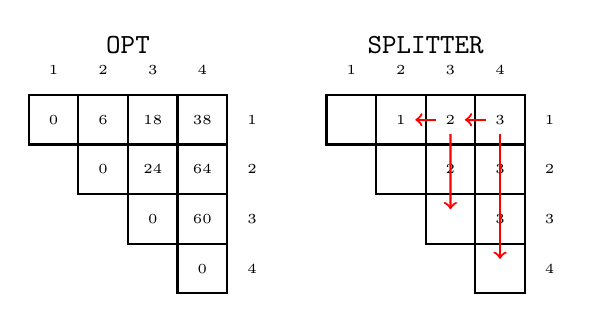
\begin{tikzpicture}[scale=0.9, auto,swap]

  	\def\d{0.7};


   	\def\d{0.7};
	
	%draw index
 \def\dy{1};
 \def\dx{0};
 \node at ( 2 * \d + \dx * \d, \dy * \d +  \d ) {\tt OPT };

    \foreach \i/\num/\name in { 1/1/s1,2/2/s2,3/3/s3,4/4/s4 }{
           \node (\name) at (\i*\d+\d/2 + \dx*\d - \d, \d/2 + \dy * \d) {\tiny $\num$};
    }

 \def\dy{0};
 \def\dx{0};
    \foreach \i/\num/\name in { 1/1/s1,2/2/s2,3/3/s3,4/4/s4 }{
         \node (\name) at ( 4*\d+\d/2  + \dx * \d,  0.0 - \i*\d + \d/2 - \dy * \d + \d){\tiny $\num$};
    }


	
 \def\dy{0};
 \def\dx{0};
    \foreach \i/\num/\name in { 0/0/s8,1/6/s7,2/18/s6,3/38/s5 }{
             \draw[  thick ] (\i*\d + \dx*\d,  0+ \dy*\d) rectangle (\i*\d+\d + \dx*\d, \d + \dy*\d);
         \node (\name) at (\i*\d+\d/2 + \dx*\d, \d/2 + \dy*\d) {\tiny $\num$};
    }
%      \draw[thick, green] (s8) circle [radius=0.3];
%      \draw[thick, blue] (s7) circle [radius=0.3];
%            \draw[thick, red] (s6) circle [radius=0.3];

 \def\dy{-1};
 \def\dx{1};
    \foreach \i/\num/\name in { 0/0/s8,1/24/s7,2/64/s6}{
             \draw[  thick ] (\i*\d + \dx*\d,  0+ \dy*\d) rectangle (\i*\d+\d + \dx*\d, \d + \dy*\d);
         \node (\name) at (\i*\d+\d/2 + \dx*\d, \d/2 + \dy*\d) {\tiny $\num$};
    }
        %  \draw[thick, green] (s6) circle [radius=0.3];

 \def\dy{-2};
 \def\dx{2};
    \foreach \i/\num/\name in { 0/0/s8,1/60/s7}{
             \draw[  thick ] (\i*\d + \dx*\d,  0+ \dy*\d) rectangle (\i*\d+\d + \dx*\d, \d + \dy*\d);
         \node (\name) at (\i*\d+\d/2 + \dx*\d, \d/2 + \dy*\d) {\tiny $\num$};
    }
            %  \draw[thick, blue] (s7) circle [radius=0.3];

     \def\dy{-3};
 \def\dx{3};
    \foreach \i/\num/\name in { 0/0/s8}{
             \draw[  thick ] (\i*\d + \dx*\d,  0+ \dy*\d) rectangle (\i*\d+\d + \dx*\d, \d + \dy*\d);
         \node (\name) at (\i*\d+\d/2 + \dx*\d, \d/2 + \dy*\d) {\tiny $\num$};
    }
         %     \draw[thick, red] (s8) circle [radius=0.3];


   %split
   	%draw index
 \def\dy{1};
 \def\dx{6};
 \node at ( 2 * \d + \dx * \d, \dy * \d +  \d ) {\tt SPLITTER};

    \foreach \i/\num/\name in { 1/1/s1,2/2/s2,3/3/s3,4/4/s4 }{
           \node (\name) at (\i*\d+\d/2 + \dx*\d - \d, \d/2 + \dy * \d) {\tiny $\num$};
    }

 \def\dy{0};
 \def\dx{6};
    \foreach \i/\num/\name in { 1/1/s1,2/2/s2,3/3/s3,4/4/s4 }{
         \node (\name) at ( 4*\d+\d/2  + \dx * \d,  0.0 - \i*\d + \d/2 - \dy * \d + \d){\tiny $\num$};
    }


	
 \def\dy{0};
 \def\dx{6};
    \foreach \i/\num/\name in { 0//s11,1/1/s12,2/2/s13,3/3/s14}{
             \draw[  thick ] (\i*\d + \dx*\d,  0+ \dy*\d) rectangle (\i*\d+\d + \dx*\d, \d + \dy*\d);
         \node (\name) at (\i*\d+\d/2 + \dx*\d, \d/2 + \dy*\d) {\tiny $\num$};
    }


 \def\dy{-1};
 \def\dx{7};
    \foreach \i/\num/\name in { 0//s21,1/2/s22,2/3/s23}{
             \draw[  thick ] (\i*\d + \dx*\d,  0+ \dy*\d) rectangle (\i*\d+\d + \dx*\d, \d + \dy*\d);
         \node (\name) at (\i*\d+\d/2 + \dx*\d, \d/2 + \dy*\d) {\tiny $\num$};
    }
 \def\dy{-2};
 \def\dx{8};
    \foreach \i/\num/\name in { 0//s31,1/3/s32}{
             \draw[  thick ] (\i*\d + \dx*\d,  0+ \dy*\d) rectangle (\i*\d+\d + \dx*\d, \d + \dy*\d);
         \node (\name) at (\i*\d+\d/2 + \dx*\d, \d/2 + \dy*\d) {\tiny $\num$};
    }
     \def\dy{-3};
 \def\dx{9};
    \foreach \i/\num/\name in { 0//s41}{
             \draw[  thick ] (\i*\d + \dx*\d,  0+ \dy*\d) rectangle (\i*\d+\d + \dx*\d, \d + \dy*\d);
         \node (\name) at (\i*\d+\d/2 + \dx*\d, \d/2 + \dy*\d) {\tiny $\num$};
    }

\draw[red, thick, ->] (s14) -- (s13);
\draw[red, thick, ->] (s14) -- (s41);
\draw[red, thick, ->] (s13) -- (s12);
\draw[red, thick, ->] (s13) -- (s31);


\end{tikzpicture}
\begin{flushleft}
第二步:    $((A_1A_2)(A_3))(A_4)$
\end{flushleft}
\end{figure}




\begin{figure}[htbp]
\centering
%\includegraphics[width=0.55\textwidth]{tree9.png}
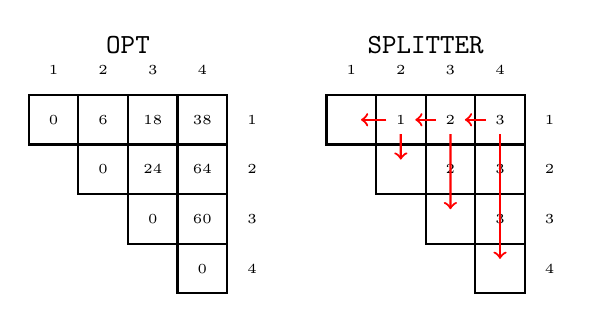
\begin{tikzpicture}[scale=0.9, auto,swap]

  	\def\d{0.7};


   	\def\d{0.7};
	
	%draw index
 \def\dy{1};
 \def\dx{0};
 \node at ( 2 * \d + \dx * \d, \dy * \d +  \d ) {\tt OPT };

    \foreach \i/\num/\name in { 1/1/s1,2/2/s2,3/3/s3,4/4/s4 }{
           \node (\name) at (\i*\d+\d/2 + \dx*\d - \d, \d/2 + \dy * \d) {\tiny $\num$};
    }

 \def\dy{0};
 \def\dx{0};
    \foreach \i/\num/\name in { 1/1/s1,2/2/s2,3/3/s3,4/4/s4 }{
         \node (\name) at ( 4*\d+\d/2  + \dx * \d,  0.0 - \i*\d + \d/2 - \dy * \d + \d){\tiny $\num$};
    }


	
 \def\dy{0};
 \def\dx{0};
    \foreach \i/\num/\name in { 0/0/s8,1/6/s7,2/18/s6,3/38/s5 }{
             \draw[  thick ] (\i*\d + \dx*\d,  0+ \dy*\d) rectangle (\i*\d+\d + \dx*\d, \d + \dy*\d);
         \node (\name) at (\i*\d+\d/2 + \dx*\d, \d/2 + \dy*\d) {\tiny $\num$};
    }
%      \draw[thick, green] (s8) circle [radius=0.3];
%      \draw[thick, blue] (s7) circle [radius=0.3];
%            \draw[thick, red] (s6) circle [radius=0.3];

 \def\dy{-1};
 \def\dx{1};
    \foreach \i/\num/\name in { 0/0/s8,1/24/s7,2/64/s6}{
             \draw[  thick ] (\i*\d + \dx*\d,  0+ \dy*\d) rectangle (\i*\d+\d + \dx*\d, \d + \dy*\d);
         \node (\name) at (\i*\d+\d/2 + \dx*\d, \d/2 + \dy*\d) {\tiny $\num$};
    }
        %  \draw[thick, green] (s6) circle [radius=0.3];

 \def\dy{-2};
 \def\dx{2};
    \foreach \i/\num/\name in { 0/0/s8,1/60/s7}{
             \draw[  thick ] (\i*\d + \dx*\d,  0+ \dy*\d) rectangle (\i*\d+\d + \dx*\d, \d + \dy*\d);
         \node (\name) at (\i*\d+\d/2 + \dx*\d, \d/2 + \dy*\d) {\tiny $\num$};
    }
            %  \draw[thick, blue] (s7) circle [radius=0.3];

     \def\dy{-3};
 \def\dx{3};
    \foreach \i/\num/\name in { 0/0/s8}{
             \draw[  thick ] (\i*\d + \dx*\d,  0+ \dy*\d) rectangle (\i*\d+\d + \dx*\d, \d + \dy*\d);
         \node (\name) at (\i*\d+\d/2 + \dx*\d, \d/2 + \dy*\d) {\tiny $\num$};
    }
         %     \draw[thick, red] (s8) circle [radius=0.3];


   %split
   	%draw index
 \def\dy{1};
 \def\dx{6};
 \node at ( 2 * \d + \dx * \d, \dy * \d +  \d ) {\tt SPLITTER};

    \foreach \i/\num/\name in { 1/1/s1,2/2/s2,3/3/s3,4/4/s4 }{
           \node (\name) at (\i*\d+\d/2 + \dx*\d - \d, \d/2 + \dy * \d) {\tiny $\num$};
    }

 \def\dy{0};
 \def\dx{6};
    \foreach \i/\num/\name in { 1/1/s1,2/2/s2,3/3/s3,4/4/s4 }{
         \node (\name) at ( 4*\d+\d/2  + \dx * \d,  0.0 - \i*\d + \d/2 - \dy * \d + \d){\tiny $\num$};
    }


	
 \def\dy{0};
 \def\dx{6};
    \foreach \i/\num/\name in { 0//s11,1/1/s12,2/2/s13,3/3/s14}{
             \draw[  thick ] (\i*\d + \dx*\d,  0+ \dy*\d) rectangle (\i*\d+\d + \dx*\d, \d + \dy*\d);
         \node (\name) at (\i*\d+\d/2 + \dx*\d, \d/2 + \dy*\d) {\tiny $\num$};
    }


 \def\dy{-1};
 \def\dx{7};
    \foreach \i/\num/\name in { 0//s21,1/2/s22,2/3/s23}{
             \draw[  thick ] (\i*\d + \dx*\d,  0+ \dy*\d) rectangle (\i*\d+\d + \dx*\d, \d + \dy*\d);
         \node (\name) at (\i*\d+\d/2 + \dx*\d, \d/2 + \dy*\d) {\tiny $\num$};
    }
 \def\dy{-2};
 \def\dx{8};
    \foreach \i/\num/\name in { 0//s31,1/3/s32}{
             \draw[  thick ] (\i*\d + \dx*\d,  0+ \dy*\d) rectangle (\i*\d+\d + \dx*\d, \d + \dy*\d);
         \node (\name) at (\i*\d+\d/2 + \dx*\d, \d/2 + \dy*\d) {\tiny $\num$};
    }
     \def\dy{-3};
 \def\dx{9};
    \foreach \i/\num/\name in { 0//s41}{
             \draw[  thick ] (\i*\d + \dx*\d,  0+ \dy*\d) rectangle (\i*\d+\d + \dx*\d, \d + \dy*\d);
         \node (\name) at (\i*\d+\d/2 + \dx*\d, \d/2 + \dy*\d) {\tiny $\num$};
    }

\draw[red, thick, ->] (s14) -- (s13);
\draw[red, thick, ->] (s14) -- (s41);

\draw[red, thick, ->] (s13) -- (s12);
\draw[red, thick, ->] (s13) -- (s31);

\draw[red, thick, ->] (s12) -- (s11);
\draw[red, thick, ->] (s12) -- (s21);

\end{tikzpicture}
\begin{flushleft}
第三步:    $(((A_1)(A_2))(A_3))(A_4)$
\end{flushleft}
\end{figure}


\newpage

根据我们的回溯,知道了最优解方案就是先算$A_1A_2$ 然后结果乘以$A_3$,最后乘以$A_4$.

\subsection{问题总结:}

经过对矩阵链式乘法的整个求解过程,我们有如下总结:

如果大问题搞不定,我们可以将其分解成更小的子问题。在动态规划求解问题时关键是如何定义子问题,
我们可以将求解过程想象成多步决策的过程,再假设已经拿到了最优解,然后考察第一个决策是做什么的,此时可能会有多种情况,那我们就枚举所有情况,然后观察子问题的所有形式,并进行总结便会得到子问题的一般形式即递归表达式。

最后看该问题是否满足最优子结构的性质。如果满足则根据递归表达式,我们便可以写出源代码。

%关于链式乘法的最优解是O($n^3$)吗?其可以转化成三角剖分问题,详见附录。。。

\section{0/1背包问题:}

现在有个物品集,每个物品都有重量和价值,现在希望选择一个物品子集,使得总的重量小于给定的重量并且总的价值最大。

\textbf{问题的形式化描述:}

该问题的形式化描述如下:

\begin{itemize}
    \item {\bf Input:}\\ A set of items. Item $i$ has weight $w_i$ and value $v_i$, and a total weight limit $W$;
	\item {\bf Output:}\\ A sub-set of items to maximize the total value with a total weight below $W$.
\end{itemize}

这里 $ 0/1$ 的意思是只能装或者不装这个物品,装记做1,不装记做0.

\indent
\subsection{具体事例:}

下面我们看下一个生活中的例子:
\begin{figure}[htbp]
\centering
%\includegraphics[width=0.55\textwidth]{017.png}
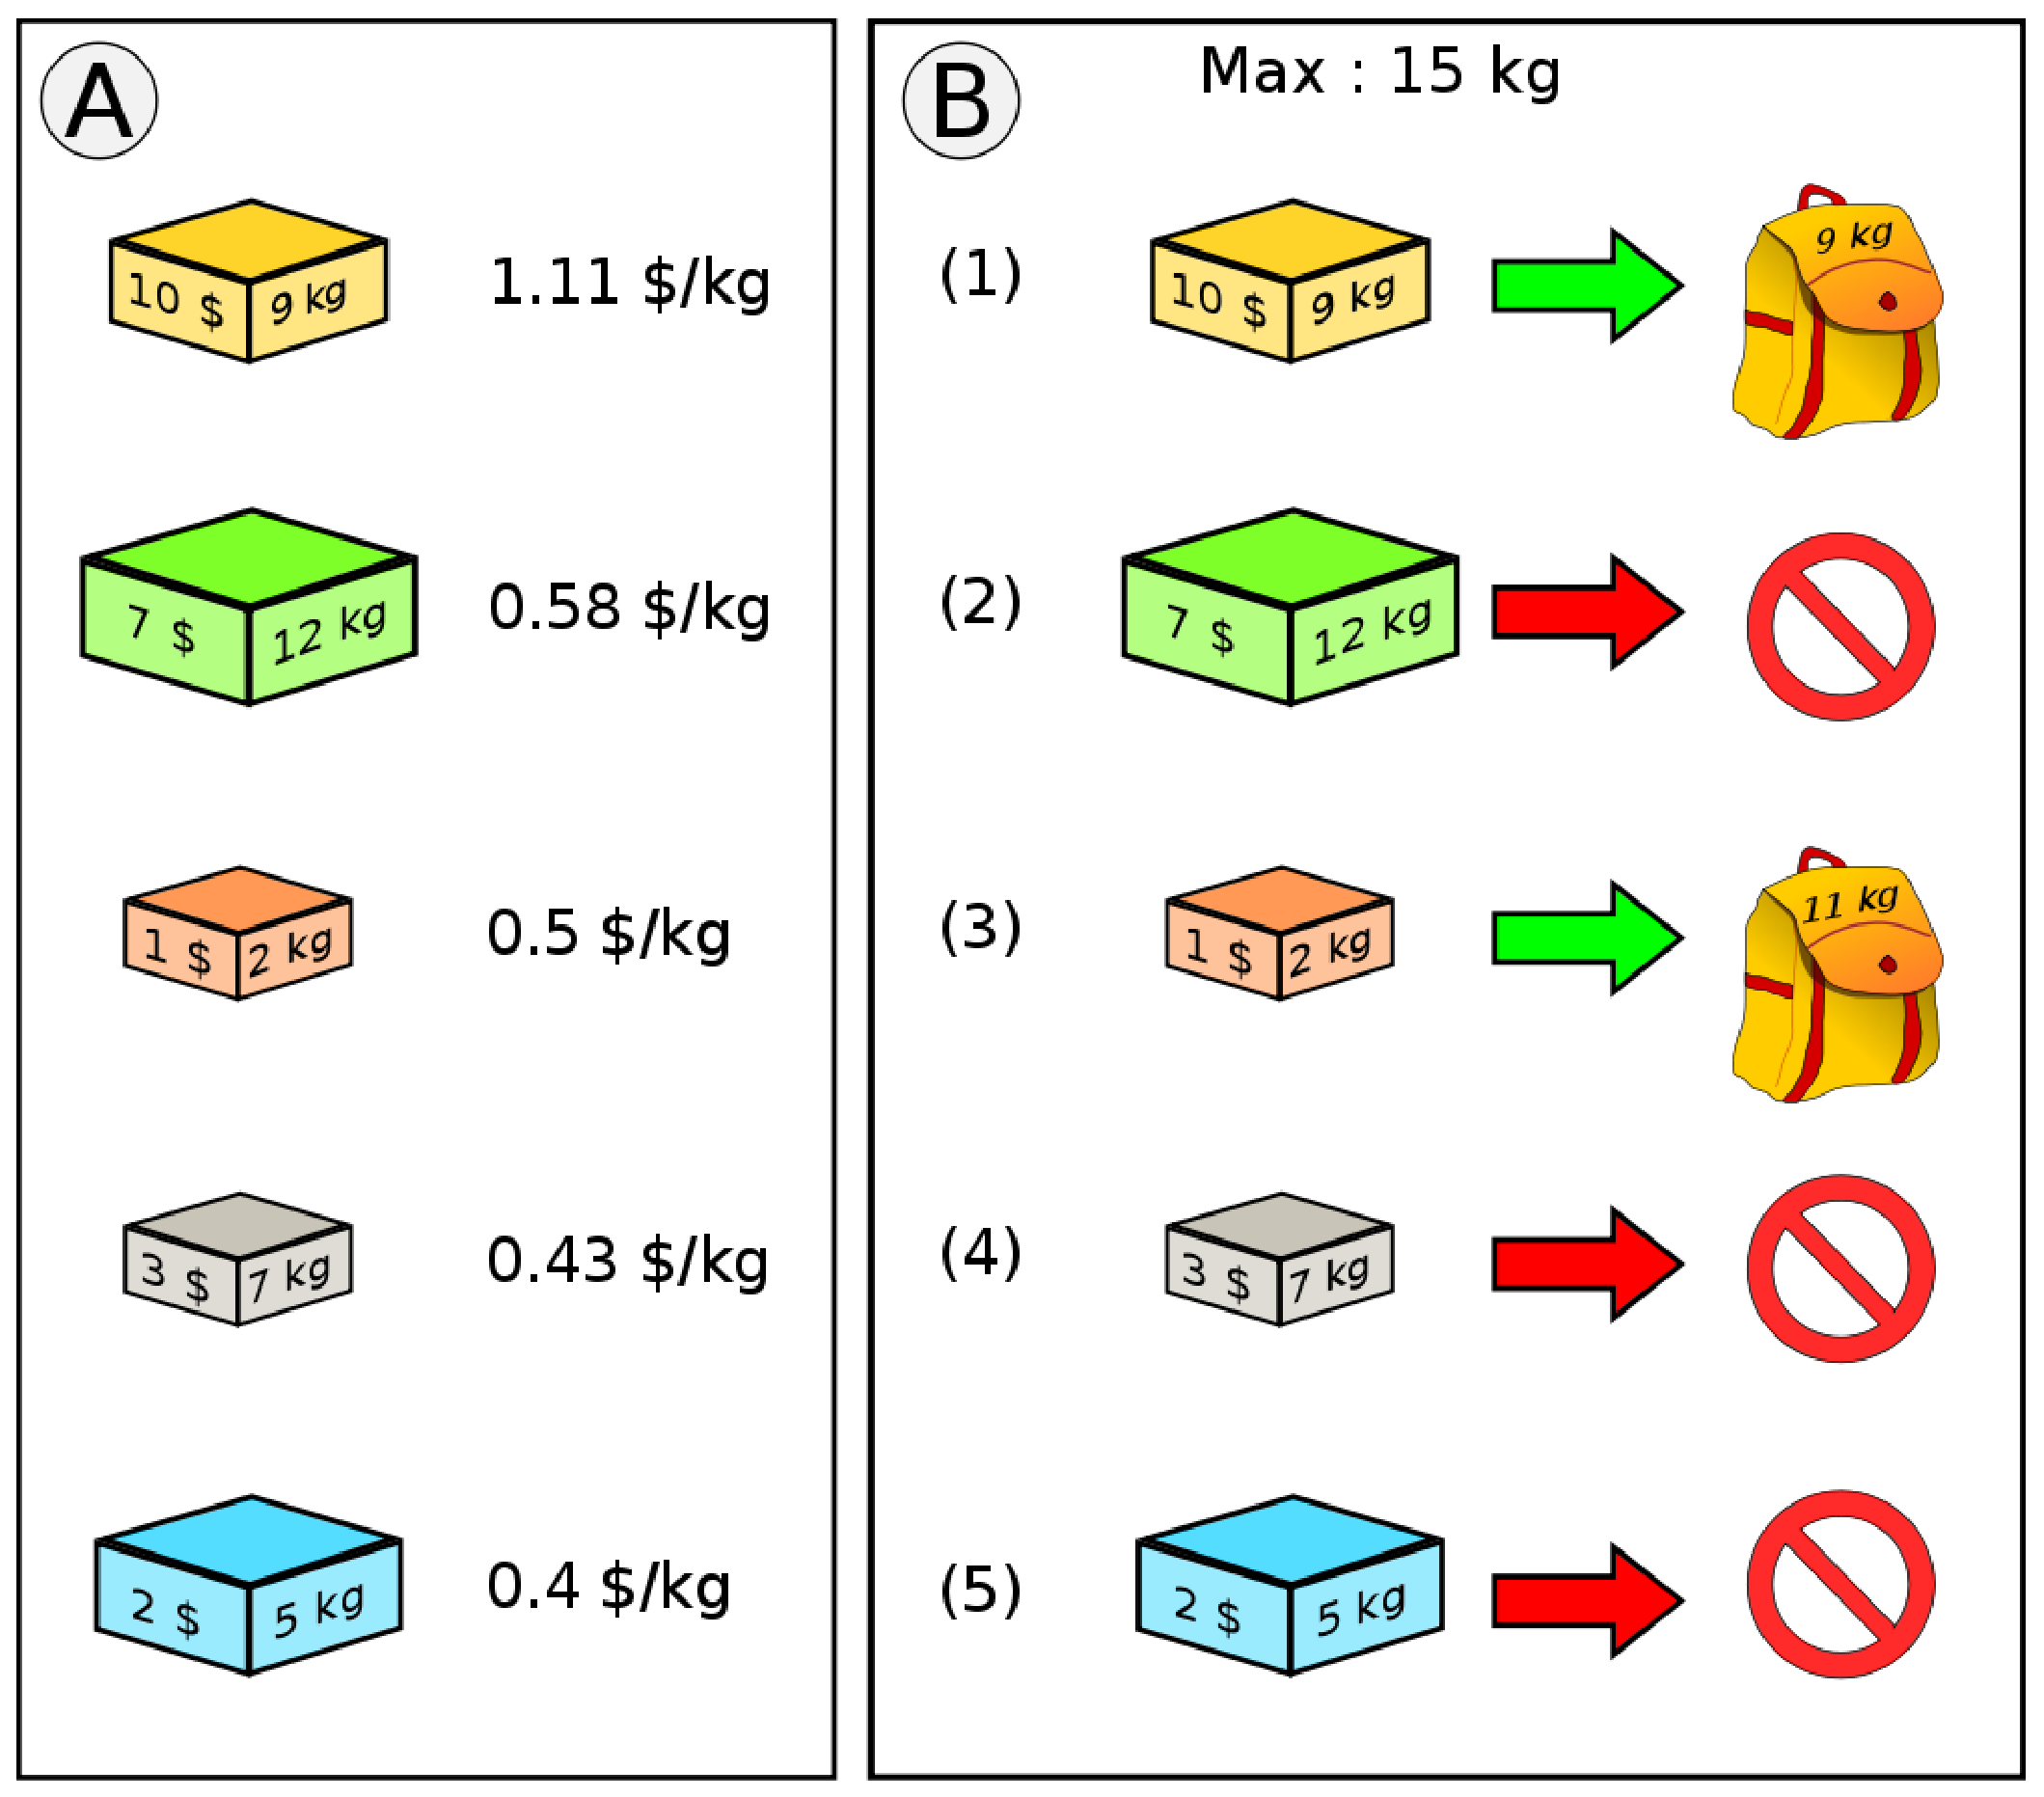
\includegraphics[width=2.3in]{1000px-Knapsack_greedy.eps}
\caption{物品从上到下依次为金银铜铁锡}

\begin{flushleft}
~~~~我们直观的想法可能是先装单价贵重的物品,比如图中的物品,我们可能会先装金块,因为最大只有15kg,装完金块后还剩6 kg,此时还能装铜块和xi块。按照我们先装单价贵重的物品则会装铜块,此时还剩下4 kg,则没有物品可以装的下了。按照我们启发式的装东西想法得到的总价为11\$,可是我们启发式得到的一定是最优的吗?下面我们看下动态规划是怎么求解的。
\end{flushleft}

\end{figure}


\subsection{动态规划求解思路:}

现在我们还是按照之前解决矩阵链式乘法的求解思路来:

当物品集是$n$个物品的时候,我们不知道怎么解决,可以先考虑$n-1$个物品,或者$n/2$个物品,看可不可以将物品数目变少。

我们解方案是选哪些物品,是物品的子集。我们可以把问题的求解想象成一系列的决策,在第 $i$ 步,我们决定第 $i$ 个物品是装还是不装。

现在假设我们已经得到子问题的最优解,当前考虑第一个决策即考虑最后一个物品是装还是不装。

如果装,则原问题变成从前$n - 1$个物品中选择限重 $W - w_n$ 的物品子集使得价值最大。

如果不装,则问题变成在前$n - 1$个物品中选择限重 $W$ 的物品子集使得价值最大。

此时对子问题的两种情况进行总结,我们可以得到子问题的一般形式,在前 $i$ 个物品中选择物品,选物品的价值越大越好,将子问题的最优解记做$OPT(i,w)$.

我们对 $(i,w)$ 的两种情况进行分析,并取最大值,则有如下递归表达式:

\[OPT( i, w )=\max\{ OPT(i-1, w), OPT(i-1, w - w_n) + v_n\}\]

根据递归表达式,我们可以写出如下伪代码:

{\sc Knapsack}$(  n, W )$
\begin{algorithmic}[1]
\FOR {$w=1$ to $W$ }
\STATE $OPT[0, w] = 0$;
\ENDFOR
\FOR {$i=1$ to $n$ }
\FOR {$w=1$ to $W$ }
\STATE $OPT[i,w] = \max \{OPT[i-1, w], v_i+OPT[i-1, w-w_i]\}$;
\ENDFOR
\ENDFOR
\end{algorithmic}


我们列了一张4行7列的一张表格, $dp[i][j]$ 表示前 $i$ 个物品,容量为 $j$ 的时候最多可以装多少价值的物品。

程序的开始需要对数组进行初始化,对前 $0$ 个物品装,无论容量多大,最大效益都是0。

因此我们有如下求解过程:

    \begin{figure}
	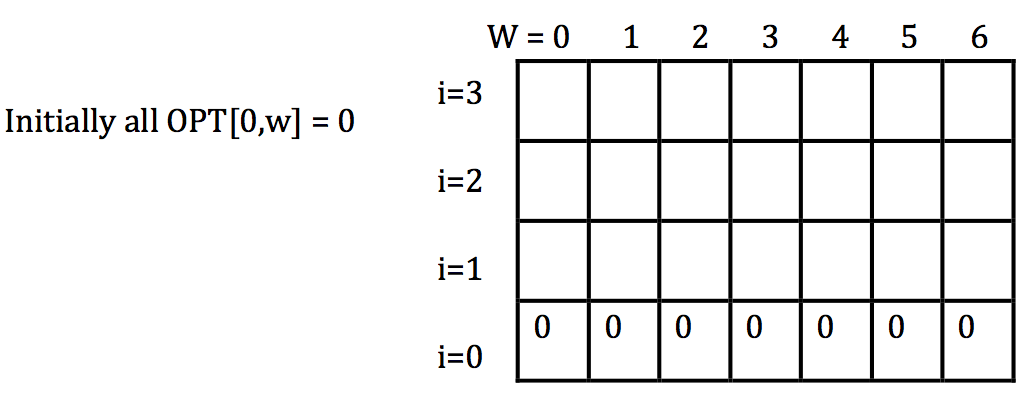
\includegraphics[width=4in]{L5-Knapsackalgostep1.png}
	\end{figure}
	\begin{figure}
	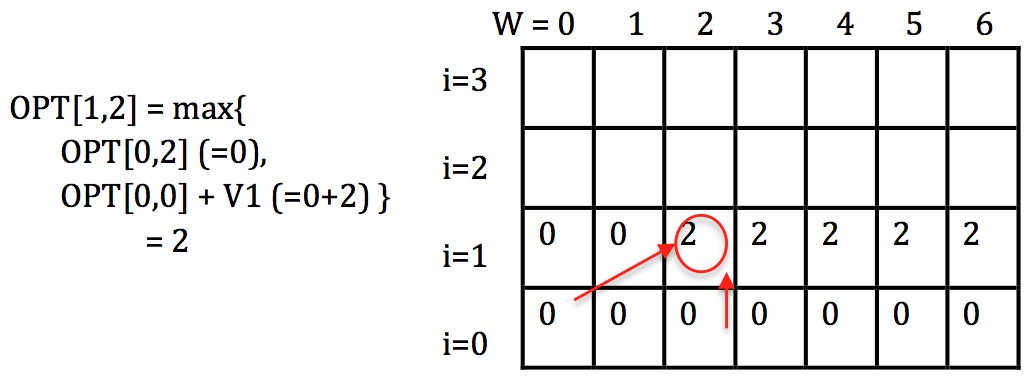
\includegraphics[width=4in]{L5-Knapsackalgostep2.png}
	\end{figure}	
	\begin{figure}
	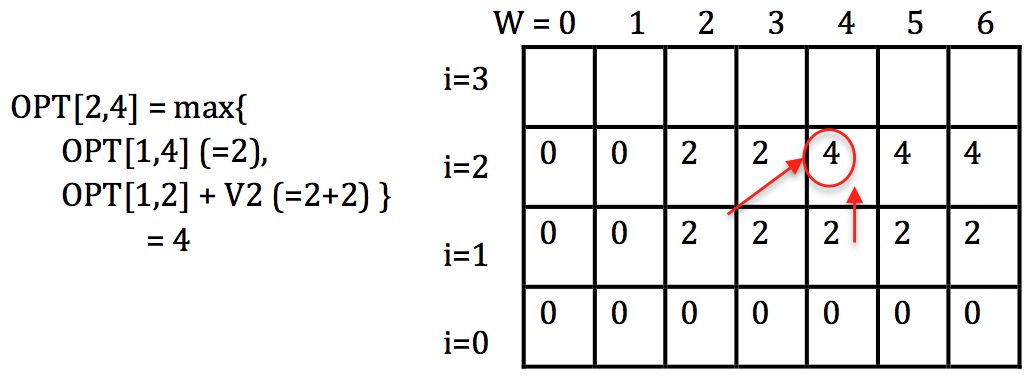
\includegraphics[width=4in]{L5-Knapsackalgostep3.png}
	\end{figure}	
	\begin{figure}
	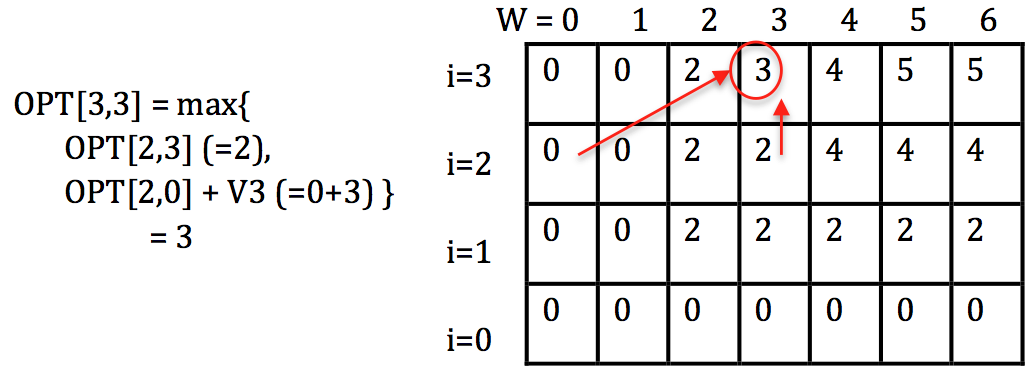
\includegraphics[width=4in]{L5-Knapsackalgostep4.png}
	\end{figure}

    Backtracking: step 1
	\begin{figure}
	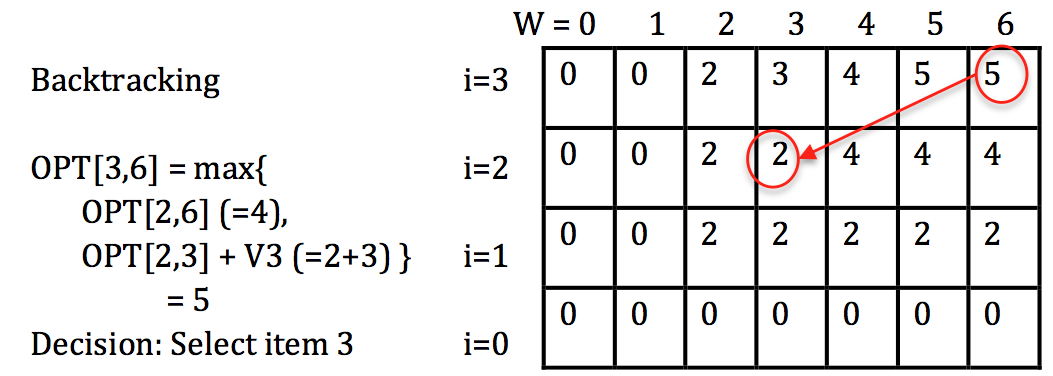
\includegraphics[width=4in]{L5-Knapsackalgobacktrackstep1.png}
	\end{figure}

    Backtracking: step 2
	\begin{figure}
	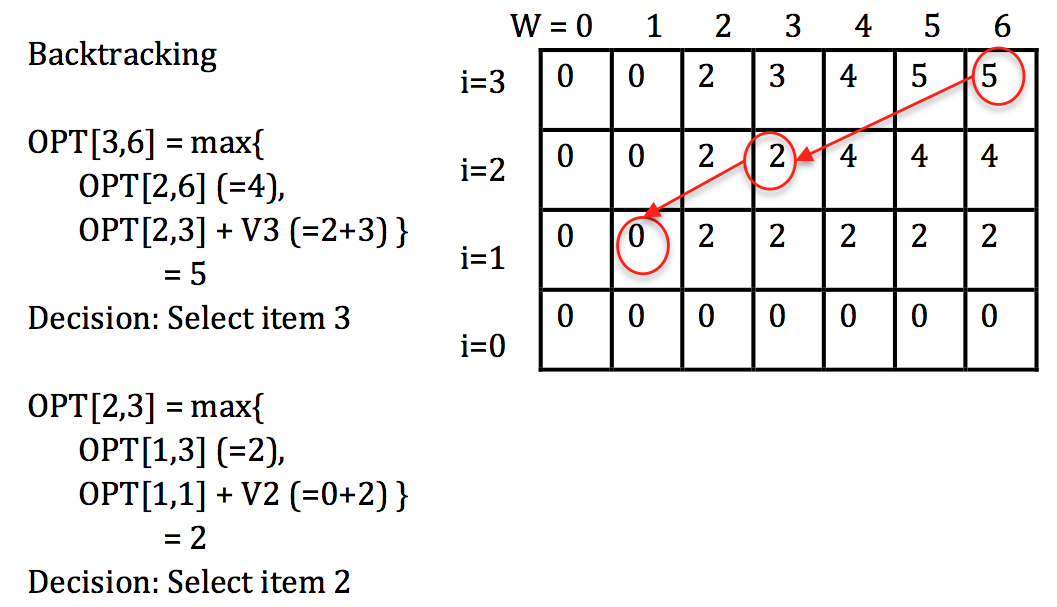
\includegraphics[width=4in]{L5-Knapsackalgobacktrackstep2.png}
	\end{figure}

\newpage

最后我们得到$dp[3][6] = 5$ ,那么如何找到最优解方案呢。

根据之前我们做矩阵链式乘法的经验知道可以通过对中间过程进行记录,一步步进行回溯找到该最优解方案。

\subsection{时间复杂度的讨论:}

该问题的时间复杂度为 $O(nW)$。因为原问题有 $nW$ 个子问题,每个子问题进行2次比较,则共有$O(2nW)$ 运算次数,因此原问题的时间复杂度就是 $O(nW)$。

如果 $W$ 过大,则该算法将不是很高效。因为数值是用2进制表示的,则 $W$ 将使用 $logW$ 个 $bit$ 表示,则原问题的时间复杂度为$O(n2^{logW}) = O(n2^{input ~ length})$, 是与输入长度相关的指数表达式, 这种形式的表达式叫做伪多项式时间的算法。

\subsection{另外一个子问题表示:}

开始我们假设所有的问题给了一个排序。现在我们假设对 $n$ 个物品不排序,则子问题可以定义成$OPT(s,W)$ 即在 $S$ 这个物品集合里,当包的容量最大是 $W$ 时如何使装的物品的价值最大。

现在考察包里面的任何一个物品,则该物品有装和不装两种情况,因此有递归表达式

\[OPT( S,W  )=\max\{ OPT(S-\{i\}, W - w_i) + v_i ~, ~ OPT(S-\{i\}, W) \}\]

这种思路在理论上是ok的,但是时间复杂度会非常高。因为任何一个物品的子集我们都要作为 $S$ 进行求解,如果有 $n$ 个物品,则有$2^n$个子集,则问题的时间复杂度将是指数级的。


而我们之前定义的 $OPT(i,w)$ 是指在前 $i$ 个物品中选且包的容量最大为 $w$ 时的装的物品价值最大。此时只考虑前 $i$ 个物品,并不考虑前 $i$ 个物品到底是哪 $i$ 个物品,则该子问题只有 $O(n)$ 个子问题,可见之前对问题的表示比上述表示要简洁的多。

可见子问题的表示对动态规划的时间复杂度有很重要的影响,如果定义的不够好将导致时间复杂度特别高。


\section{序列的连配问题}

\subsection{问题描述:}

关于序列连配问题的实际需求比较多,比如生物信息领域中DNA序列的匹配问题。生活中常见的例子就是我们在word里面打英文单词,如果有错误,它会划红线进行提醒,有时甚至可以自动修改。

关于判断输入的英文单词是否错误,我们可以在系统后台存储一个词典。如果打出的英文单词不在该词典中,则该词就判断为错误,但是如何自动化修改呢?如何知道该词与词典中的哪个词最近呢?比如我们敲入的是teh这个单词,如何自动修改成the这个单词呢?

关键问题在于如何评判键盘敲入的单词与词典背后的单词的相似程度呢?比如我们敲入的是OCURRANCE这个单词,我们通过插入一个字母C和修改A这个字母为E变成词典中的OCCURRENCE这个单词,即我们可以经过有限次的修改,删除,添加操作,可以将敲出的单词变成词典中某个正确的单词。

\subsection{形式化定义:}

因此我们引出序列连配问题的形式化定义:

\begin{itemize}
    \item {\bf Input:}\\ Two sequence $S$ and $T$, $|S|=m$, and $|T|=n$;
	\item {\bf Output:}\\  To identify an alignment of $S$ and $T$ that maximizes a scoring function.
	\\
	
	Note: for the sake of simplicity, the following indexing schema is used: $S=S_1S_2...S_m$.
\end{itemize}

这里Alignment是左右对齐的意思,经常表示产生式过程,表示上面的单词S是怎样通过下面的单词T变成的。

我们的目标就是通过添加空格使上下序列一样长,例如在S中添加一些空格变成S’,T中添加一些空格变成T‘。

如果变了之后T‘的第i个是空格,则表示S该位置上的字母是T通过插入操作得到的。

如果变了之后S‘的第i个是空格,则表示S是将T中该位置的字母删除了。

因此Alignment就是记录了T是经过怎样一系列的变化变成S的。

现在假设我们有两个序列: S : teh 和 T: the

我们认为敲的S与字典里面的T是最相似的。为什么最相似呢,肯定是我们对单词之间的相似度进行了打分,那怎么打分的呢?

我们假设有如下打分原则:

\[
d(S,T)=\sum_{i=1}^{|S'|} \delta( S'[i], T'[i] )
\]

这里的 $\delta(a,b)$ is:
\begin{enumerate}
 \item Match: +1 , e.g.  $\delta(`C', `C') = 1$.\\
 \item Mismatch: -1, e.g.  $\delta(`E', `A') = -1$.\\
 \item Ins/Del: -3, e.g.  $\delta(`C', `-') = -3$.\\
\end{enumerate}

$\delta(a,b)$ 表示如果当前S位置上的字母与T位置上的字母match到了,则+1分,如果没有match到则-1分,少敲则-3分。这里这样设计打分原则只是为了教学方便。

一个问题可以建模成组合优化或者统计问题,这两个问题是密切相关的。

使用Alignment,我们可以知道你最想敲的是什么。我们系统后台有个词典,词典中的每个单词都与你想敲的单词进行相似度计算,则找到与你敲的单词最相似的就是你最想敲的,也就是得分最高的那个单词。

\textbf{
具体事例:}

例如下面一个例子:

\begin{itemize}
\item 
\begin{enumerate}
\item $T=$``\texttt{OCCUPATION}'':
\begin{figure}
	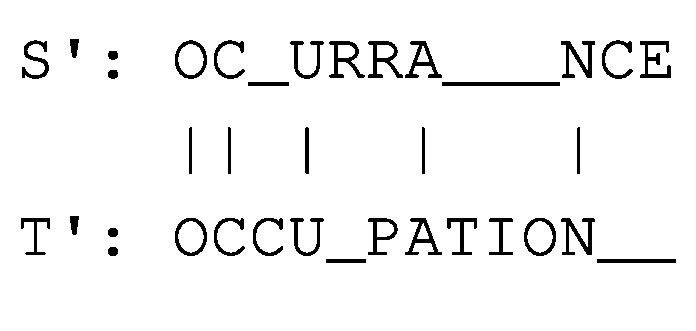
\includegraphics[width=1.4in]{L6-ocurrance-occupation-align.eps}
\end{figure}
$d(S',T') = 1+1-3+1-3-3-1+1-3-3-3+1-3-3 = -28$.
\item $T=``$\texttt{OCCURRENCE}'':
\begin{figure}
	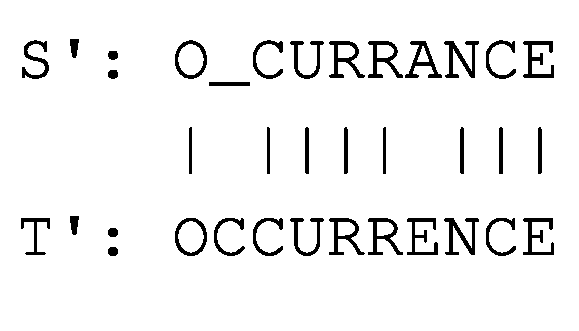
\includegraphics[width=1.3in]{L6-ocurrance-occurrence-align1.eps}
\end{figure}
$d(S',T') = 1-3+1+1+1+1-1+1+1+1 =4$.
\end{enumerate}
\item
\begin{flushleft}
    ~~~~我们对单词“OCCUPATION”和“OCURRANCE”通过加空格使得它们等长,然后通过计分的方案得到“OCCUPATION” 与“OCURRANCE”的得分是-28 分。
    \end{flushleft}

    \begin{flushleft}
    ~~~~同样假设我们在词典中遇到了另外一个词“OCCURRENCE”,和上面一样操作,最后得到“OCCURRENCE” 与“OCURRANCE” 的得分是4 分。
    \end{flushleft}
\end{itemize}


%\begin{figure}
	%\centering
	%\includegraphics[width=4.4in]{alignment1.png}   
%\end{figure}

\newpage
因为单词“OCCURRENCE”得分比较高,所以我们猜测敲错的单词“OCURRANCE”极有可能是从“OCCURRENCE”这个单词过来的。

另外我们还能知道你是怎么敲的?

即使我们找到与“OCURRANCE”最相似的是“OCCURRENCE”这个单词,我们仍然有很多种加空格的方案使得他们等长。

\begin{itemize}
\item
\begin{enumerate}
\item Alignment 1:
\begin{figure}
	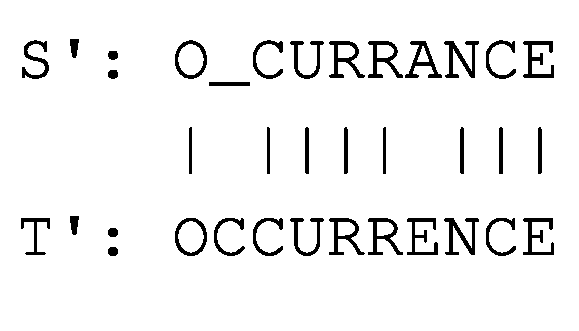
\includegraphics[width=1.3in]{L6-ocurrance-occurrence-align1.eps}
\end{figure}
$d(S',T') = 1-3+1+1+1+1-1+1+1+1 =4$.
\item Alignment 2:
\begin{figure}
	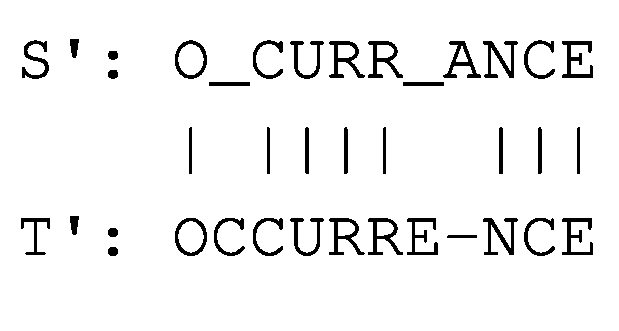
\includegraphics[width=1.3in]{L6-ocurrance-occurrence-align2.eps}
\end{figure}
$d(S',T') = 1-3+1+1+1-3-3+1+1+1=-1$.
\end{enumerate}

\item
    \begin{flushleft}
    ~~~~这两种加空格的方案都可以使得单词“OCURRANCE”与”OCCURRENCE“等长,但是得分却是不同的。通过Alignment 我们可以知道单词”OCURRANCE“中的字母A 最可能是把字母E 敲错了得到的,而不是少敲了一个E且多敲了一个A得到的。
    \end{flushleft}
\end{itemize}


%\begin{figure}
	%\centering
	%\includegraphics[width=4.4in]{alignment17.png} 
%\end{figure}

\newpage
因此我们知道Alignment十分重要,不仅可以识别出字典中哪个单词与你敲的单词相似度最大,而且可以推测出你是怎么敲错的。

\subsection{动态规划求解:}

现在我们对问题进行总结:

给我们两个字符串S与T,问如何通过加空格使得得分最高。

采用我们之前求解问题的一般思路:首先给我们的字符串很长,我们不好解决,我们可以将该字符串分成更小的字符串,我们的solution是通过加空格使两个字符串对齐的方案。我们把求解过程当做一系列的决策,对每个决策部分我们决定 $s[i]$  是怎样通过 $T[j]$ 变来的,比如$OCURRANCE$是S,$OCCURRENCE$是T,我们尝试考虑 $S$ 是经过什么样的操作变化到 $T$ 的。

我们首先考虑S单词最后的字母E,那S的E是通过T怎么变化得到的呢?

(1)从T的最后一个单词直接过来的,即 match 到了。

(2)这个E是我们多敲的,即T通过插入操作变化过来的。

(3)这个E是我们少敲的,即T通过删除操作变化过来的。

我们的总体目标是给我们一个词,我们想知道该词是否与词典中的某个词相似,给我们的词太长不好解决,可以先考虑最后一个字母,看它有哪些来源。

如果是多敲的,则S除了最后一个字母剩余的部分,是由T的整体变化而来的。则问题变成假设我们找到一个最优解,现在我们只考虑最后一个决策,即S的最后一个字母是怎么过来的呢?我们由上面的分析知道,其来源三种可能。


(1)如果S[m]与T[n]形成匹配,则子问题变成了 $S[1,...,m-1] $ 与 $T[1,..,n - 1]$ 的对齐问题。

(2)如果S[m]与空格匹配,则表示S[m] 是T通过插入操作过来的,则子问题变成了 $S[1,...,m-1] $ 与 $T[1,..,n ]$ 的对齐问题。

(3)如果T[n]与空格匹配,则表示S[m] 是T通过删除操作过来的,则子问题变成了 $S[1,...,m] $ 与 $T[1,..,n - 1]$ 的对齐问题。

则我们可以总结得到子问题的一般形式就是S的前缀与T的前缀的对齐方案,我们将该问题的最优解记做$OPT(i,j) =  S[1...i] ~ alignment ~ T[1...j]$.

因此我们可以得到如下递归表达式:

\begin{small}
$OPT( i, j) = \max \begin{cases} \delta(S_i, T_j) + OPT(i-1, j-1) &  \\
 \delta(`\_', T_j) + OPT(i, j-1) & \\
 \delta(S_i,`\_') + OPT(i-1,j)
\end{cases}$
\end{small}

即枚举当前单元的三种可能来源,在其中取最大值就可以。

因此有如下伪代码:
\\

{\sc Needleman\_Wunch}$( S, T )$
\begin{algorithmic}[1]
\FOR {$i=0$ to $m$;}
\STATE $OPT[i,0] = -3*i;$
\ENDFOR
\FOR {$j=0$ to $n$; }
\STATE $OPT[0,j] = -3*j;$
\ENDFOR
\FOR {$i=1$ to $m$  }
\FOR {$j=1$ to $n$  }
\STATE $OPT[i,j] = \max \{OPT[i-1, j-1] + \delta(S_i,T_j), OPT[i-1, j] - 3, OPT[i, j-1] - 3\};$
\ENDFOR
\ENDFOR
\RETURN {$OPT[m,n]$ };
\end{algorithmic}

Note: the first row is introduced to describe the alignment of prefixes $T[1..i]$ with an empty sequence $\epsilon$, so does the first column.

\begin{figure}
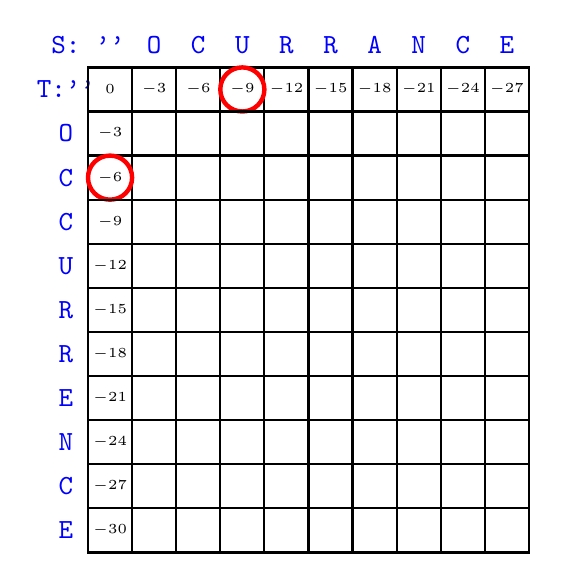
\begin{tikzpicture}[scale=0.8, auto,swap]

  	\def\d{0.7};
	
	%draw index
 \def\dy{1};
 \def\dx{0};

    \foreach \i/\num/\name in { 0/S:\ /, 1/''/s1,2/O/s2,3/C/s3,4/U/s4,5/R/,6/R/,7/A/,8/N/,9/C/,10/E/}{
           \node[blue,thick] (\name) at (\i*\d+\d/2 + \dx*\d - \d, \d/2 + \dy * \d) {\tt \num};
    }

 \def\dy{0};
 \def\dx{0};
    \foreach \i/\num/\name in { 1/T:''/s1,2/O/s2,3/C/s3,4/C/s4, 5/U/,6/R/,7/R/,8/E/,9/N/,10/C/,11/E/}{
         \node[blue,thick] (\name) at ( -1*\d+\d/2,  0.0 - \i*\d + \d/2 - \dy * \d + \d){\tt  \num};
    }


%score	
 \def\dy{0};
 \def\dx{0};
    \foreach \i/\num/\name in { 0/0/,1/-3/,2/-6/,3/-9/S3,4/-12/,5/-15/,6/-18/,7/-21/,8/-24/,9/-27/}{
             \draw[  thick ] (\i*\d + \dx*\d,  0+ \dy*\d) rectangle (\i*\d+\d + \dx*\d, \d + \dy*\d);
         \node (\name) at (\i*\d+\d/2 + \dx*\d, \d/2 + \dy*\d) {\tiny $\num$};
    }
 \draw[red,ultra thick] (S3) circle[radius=\d/2];

 \def\dy{-1};
 \def\dx{0};
    \foreach \i/\num/\name in { 0/-3/,1//,2//,3//S3,4//,5//,6//,7//,8//,9//}{
             \draw[  thick ] (\i*\d + \dx*\d,  0+ \dy*\d) rectangle (\i*\d+\d + \dx*\d, \d + \dy*\d);
         \node (\name) at (\i*\d+\d/2 + \dx*\d, \d/2 + \dy*\d) {\tiny $\num$};
    }

 \def\dy{-2};
 \def\dx{0};
    \foreach \i/\num/\name in { 0/-6/S0,1//,2//,3//S3,4//,5//,6//,7//,8//,9//}{
             \draw[  thick ] (\i*\d + \dx*\d,  0+ \dy*\d) rectangle (\i*\d+\d + \dx*\d, \d + \dy*\d);
         \node (\name) at (\i*\d+\d/2 + \dx*\d, \d/2 + \dy*\d) {\tiny $\num$};
    }
     \draw[red,ultra thick] (S0) circle[radius=\d/2];

 \def\dy{-3};
 \def\dx{0};
    \foreach \i/\num/\name in { 0/-9/,1//,2//,3//S3,4//,5//,6//,7//,8//,9//}{
             \draw[  thick ] (\i*\d + \dx*\d,  0+ \dy*\d) rectangle (\i*\d+\d + \dx*\d, \d + \dy*\d);
         \node (\name) at (\i*\d+\d/2 + \dx*\d, \d/2 + \dy*\d) {\tiny $\num$};
    }

  \def\dy{-4};
 \def\dx{0};
    \foreach \i/\num/\name in { 0/-12/,1//,2//,3//S3,4//,5//,6//,7//,8//,9//}{
             \draw[  thick ] (\i*\d + \dx*\d,  0+ \dy*\d) rectangle (\i*\d+\d + \dx*\d, \d + \dy*\d);
         \node (\name) at (\i*\d+\d/2 + \dx*\d, \d/2 + \dy*\d) {\tiny $\num$};
    }

  \def\dy{-5};
 \def\dx{0};
    \foreach \i/\num/\name in { 0/-15/,1//,2//,3//S3,4//,5//,6//,7//,8//,9//}{
             \draw[  thick ] (\i*\d + \dx*\d,  0+ \dy*\d) rectangle (\i*\d+\d + \dx*\d, \d + \dy*\d);
         \node (\name) at (\i*\d+\d/2 + \dx*\d, \d/2 + \dy*\d) {\tiny $\num$};
    }

  \def\dy{-6};
 \def\dx{0};
    \foreach \i/\num/\name in { 0/-18/,1//,2//,3//S3,4//,5//,6//,7//,8//,9//}{
             \draw[  thick ] (\i*\d + \dx*\d,  0+ \dy*\d) rectangle (\i*\d+\d + \dx*\d, \d + \dy*\d);
         \node (\name) at (\i*\d+\d/2 + \dx*\d, \d/2 + \dy*\d) {\tiny $\num$};
    }

  \def\dy{-7};
 \def\dx{0};
    \foreach \i/\num/\name in { 0/-21/,1//,2//,3//S3,4//,5//,6//,7//,8//,9//}{
             \draw[  thick ] (\i*\d + \dx*\d,  0+ \dy*\d) rectangle (\i*\d+\d + \dx*\d, \d + \dy*\d);
         \node (\name) at (\i*\d+\d/2 + \dx*\d, \d/2 + \dy*\d) {\tiny $\num$};
    }

  \def\dy{-8};
 \def\dx{0};
    \foreach \i/\num/\name in { 0/-24/,1//,2//,3//S3,4//,5//,6//,7//,8//,9//}{
             \draw[  thick ] (\i*\d + \dx*\d,  0+ \dy*\d) rectangle (\i*\d+\d + \dx*\d, \d + \dy*\d);
         \node (\name) at (\i*\d+\d/2 + \dx*\d, \d/2 + \dy*\d) {\tiny $\num$};
    }

  \def\dy{-9};
 \def\dx{0};
    \foreach \i/\num/\name in { 0/-27/,1//,2//,3//S3,4//,5//,6//,7//,8//,9//}{
             \draw[  thick ] (\i*\d + \dx*\d,  0+ \dy*\d) rectangle (\i*\d+\d + \dx*\d, \d + \dy*\d);
         \node (\name) at (\i*\d+\d/2 + \dx*\d, \d/2 + \dy*\d) {\tiny $\num$};
    }

  \def\dy{-10};
 \def\dx{0};
    \foreach \i/\num/\name in { 0/-30/,1//,2//,3//S3,4//,5//,6//,7//,8//,9//}{
             \draw[  thick ] (\i*\d + \dx*\d,  0+ \dy*\d) rectangle (\i*\d+\d + \dx*\d, \d + \dy*\d);
         \node (\name) at (\i*\d+\d/2 + \dx*\d, \d/2 + \dy*\d) {\tiny $\num$};
    }





\end{tikzpicture}
\end{figure}
 \begin{tiny}

  \begin{table}
  \begin{tabular}{ll||ll}
  Score:  & \texttt{ d("OCU", "") = -9 }  & Score:  & \texttt{ d("", "OC") = -6 }  \\
  Alignment:  &  \texttt{  S'=  OCU }  & Alignment:  &  \texttt{  S'=  -- } \\
		    &	\texttt{ T'=  --- }  &   &	\texttt{ T'=  OC } \\
  \end{tabular}
  \end{table}

  \end{tiny}

我们通过伪代码可以得到下面的表格,S中每个字母一列,T中每个字母一行,其中单元 $(i,j)$ 表示$S[1,...,j]$ 与 $T[1,...,i]$ 对齐所能得到的最大的分数,比如图中的单元(1,2):


\begin{figure}
	\centering
	%\includegraphics[width=4.2in]{alignment21.png}
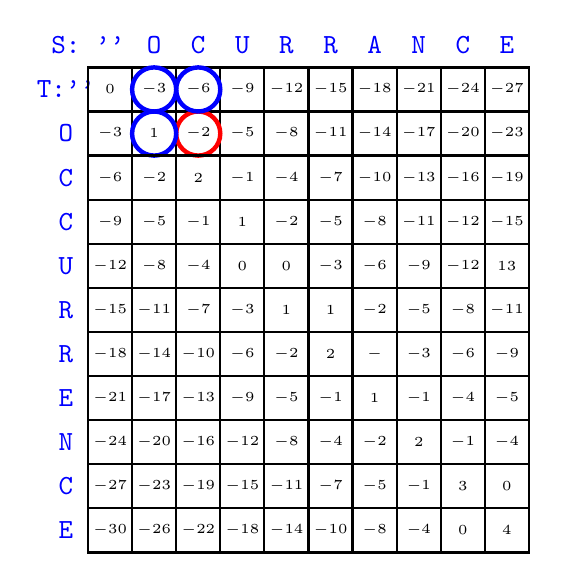
\begin{tikzpicture}[scale=0.8, auto,swap]

  	\def\d{0.7};
	
	%draw index
 \def\dy{1};
 \def\dx{0};

    \foreach \i/\num/\name in { 0/S:\ /, 1/''/s1,2/O/s2,3/C/s3,4/U/s4,5/R/,6/R/,7/A/,8/N/,9/C/,10/E/}{
           \node[blue,thick] (\name) at (\i*\d+\d/2 + \dx*\d - \d, \d/2 + \dy * \d) {\tt \num};
    }

 \def\dy{0};
 \def\dx{0};
    \foreach \i/\num/\name in { 1/T:''/s1,2/O/s2,3/C/s3,4/C/s4, 5/U/,6/R/,7/R/,8/E/,9/N/,10/C/,11/E/}{
         \node[blue,thick] (\name) at ( -1*\d+\d/2,  0.0 - \i*\d + \d/2 - \dy * \d + \d){\tt  \num};
    }


%score	
 \def\dy{0};
 \def\dx{0};
    \foreach \i/\num/\name in { 0/0/,1/-3/S1,2/-6/S2,3/-9/,4/-12/,5/-15/,6/-18/,7/-21/,8/-24/,9/-27/}{
             \draw[  thick ] (\i*\d + \dx*\d,  0+ \dy*\d) rectangle (\i*\d+\d + \dx*\d, \d + \dy*\d);
         \node (\name) at (\i*\d+\d/2 + \dx*\d, \d/2 + \dy*\d) {\tiny $\num$};
    }


 \def\dy{-1};
 \def\dx{0};
    \foreach \i/\num/\name in { 0/-3/,1/1/L,2/-2/C,3/-5/,4/-8/,5/-11/,6/-14/,7/-17/,8/-20/,9/-23/}{
             \draw[  thick ] (\i*\d + \dx*\d,  0+ \dy*\d) rectangle (\i*\d+\d + \dx*\d, \d + \dy*\d);
         \node (\name) at (\i*\d+\d/2 + \dx*\d, \d/2 + \dy*\d) {\tiny $\num$};
    }

    \draw[red,ultra thick] (C) circle[radius=\d/2];
   \draw[blue,ultra thick] (S1) circle[radius=\d/2];
   \draw[blue,ultra thick] (S2) circle[radius=\d/2];
   \draw[blue,ultra thick] (L) circle[radius=\d/2];



 \def\dy{-2};
 \def\dx{0};
    \foreach \i/\num/\name in { 0/-6/,1/-2/,2/2/,3/-1/S3,4/-4/,5/-7/,6/-10/,7/-13/,8/-16/,9/-19/}{
             \draw[  thick ] (\i*\d + \dx*\d,  0+ \dy*\d) rectangle (\i*\d+\d + \dx*\d, \d + \dy*\d);
         \node (\name) at (\i*\d+\d/2 + \dx*\d, \d/2 + \dy*\d) {\tiny $\num$};
    }

 \def\dy{-3};
 \def\dx{0};
    \foreach \i/\num/\name in { 0/-9/,1/-5/,2/-1/,3/1/S3,4/-2/,5/-5/,6/-8/,7/-11/,8/-12/,9/-15/}{
             \draw[  thick ] (\i*\d + \dx*\d,  0+ \dy*\d) rectangle (\i*\d+\d + \dx*\d, \d + \dy*\d);
         \node (\name) at (\i*\d+\d/2 + \dx*\d, \d/2 + \dy*\d) {\tiny $\num$};
    }

  \def\dy{-4};
 \def\dx{0};
    \foreach \i/\num/\name in { 0/-12/,1/-8/,2/-4/,3/0/S3,4/0/,5/-3/,6/-6/,7/-9/,8/-12/,9/13/}{
             \draw[  thick ] (\i*\d + \dx*\d,  0+ \dy*\d) rectangle (\i*\d+\d + \dx*\d, \d + \dy*\d);
         \node (\name) at (\i*\d+\d/2 + \dx*\d, \d/2 + \dy*\d) {\tiny $\num$};
    }

  \def\dy{-5};
 \def\dx{0};
    \foreach \i/\num/\name in { 0/-15/,1/-11/,2/-7/,3/-3/S3,4/1/,5/1/,6/-2/,7/-5/,8/-8/,9/-11/}{
             \draw[  thick ] (\i*\d + \dx*\d,  0+ \dy*\d) rectangle (\i*\d+\d + \dx*\d, \d + \dy*\d);
         \node (\name) at (\i*\d+\d/2 + \dx*\d, \d/2 + \dy*\d) {\tiny $\num$};
    }

  \def\dy{-6};
 \def\dx{0};
    \foreach \i/\num/\name in { 0/-18/,1/-14/,2/-10/,3/-6/S3,4/-2/,5/2/,6/-/,7/-3/,8/-6/,9/-9/}{
             \draw[  thick ] (\i*\d + \dx*\d,  0+ \dy*\d) rectangle (\i*\d+\d + \dx*\d, \d + \dy*\d);
         \node (\name) at (\i*\d+\d/2 + \dx*\d, \d/2 + \dy*\d) {\tiny $\num$};
    }

  \def\dy{-7};
 \def\dx{0};
    \foreach \i/\num/\name in { 0/-21/,1/-17/,2/-13/,3/-9/S3,4/-5/,5/-1/,6/1/,7/-1/,8/-4/,9/-5/}{
             \draw[  thick ] (\i*\d + \dx*\d,  0+ \dy*\d) rectangle (\i*\d+\d + \dx*\d, \d + \dy*\d);
         \node (\name) at (\i*\d+\d/2 + \dx*\d, \d/2 + \dy*\d) {\tiny $\num$};
    }

  \def\dy{-8};
 \def\dx{0};
    \foreach \i/\num/\name in { 0/-24/,1/-20/,2/-16/,3/-12/S3,4/-8/,5/-4/,6/-2/,7/2/,8/-1/,9/-4/}{
             \draw[  thick ] (\i*\d + \dx*\d,  0+ \dy*\d) rectangle (\i*\d+\d + \dx*\d, \d + \dy*\d);
         \node (\name) at (\i*\d+\d/2 + \dx*\d, \d/2 + \dy*\d) {\tiny $\num$};
    }

  \def\dy{-9};
 \def\dx{0};
    \foreach \i/\num/\name in { 0/-27/,1/-23/,2/-19/,3/-15/S3,4/-11/,5/-7/,6/-5/,7/-1/,8/3/,9/0/}{
             \draw[  thick ] (\i*\d + \dx*\d,  0+ \dy*\d) rectangle (\i*\d+\d + \dx*\d, \d + \dy*\d);
         \node (\name) at (\i*\d+\d/2 + \dx*\d, \d/2 + \dy*\d) {\tiny $\num$};
    }

  \def\dy{-10};
 \def\dx{0};
    \foreach \i/\num/\name in { 0/-30/,1/-26/,2/-22/,3/-18/S3,4/-14/,5/-10/,6/-8/,7/-4/,8/0/,9/4/}{
             \draw[  thick ] (\i*\d + \dx*\d,  0+ \dy*\d) rectangle (\i*\d+\d + \dx*\d, \d + \dy*\d);
         \node (\name) at (\i*\d+\d/2 + \dx*\d, \d/2 + \dy*\d) {\tiny $\num$};
    }

\end{tikzpicture}
\end{figure}

 \begin{tiny}
  \begin{table}
  \begin{tabular}{lll}

  Score:  & \texttt{ d("OC", "O") = } $  \max \left \{  \begin{array}{lll} \text{ d(``OC``,````) } & -3  & \text{ (=-9) } \\
  													\text{ d(``O``,````) }      & -1  & \text{ (=-4) } \\
													\text{ d(``O``,``O``) }   &  -3 & \text{ (=-2) } \end{array} \right.  $       \\
    Alignment:  &  \texttt{  S'=  OC } \\
   		     &	\texttt{ T'=  O- } \\
  \end{tabular}
  \end{table}
  \end{tiny}

\begin{flushleft}
~~~~单元(1,2)表示将T的前缀O敲成S的前缀OC时的Alignment情况,根据之前的分析我们知道有上述三个来源,即$(1,2)$单元仅与 $(1,1),(0,2),(0,1)$ 这三个单元有关。
\end{flushleft}


\begin{figure}
	\centering
	%\includegraphics[width=4.4in]{alignment22.png}
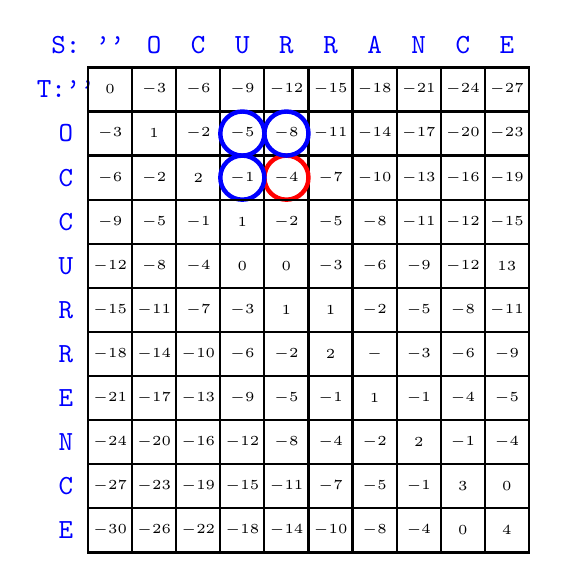
\begin{tikzpicture}[scale=0.8, auto,swap]

  	\def\d{0.7};
	
	%draw index
 \def\dy{1};
 \def\dx{0};

    \foreach \i/\num/\name in { 0/S:\ /, 1/''/s1,2/O/s2,3/C/s3,4/U/s4,5/R/,6/R/,7/A/,8/N/,9/C/,10/E/}{
           \node[blue,thick] (\name) at (\i*\d+\d/2 + \dx*\d - \d, \d/2 + \dy * \d) {\tt \num};
    }

 \def\dy{0};
 \def\dx{0};
    \foreach \i/\num/\name in { 1/T:''/s1,2/O/s2,3/C/s3,4/C/s4, 5/U/,6/R/,7/R/,8/E/,9/N/,10/C/,11/E/}{
         \node[blue,thick] (\name) at ( -1*\d+\d/2,  0.0 - \i*\d + \d/2 - \dy * \d + \d){\tt  \num};
    }


%score	
 \def\dy{0};
 \def\dx{0};
    \foreach \i/\num/\name in { 0/0/,1/-3/S1,2/-6/S2,3/-9/,4/-12/,5/-15/,6/-18/,7/-21/,8/-24/,9/-27/}{
             \draw[  thick ] (\i*\d + \dx*\d,  0+ \dy*\d) rectangle (\i*\d+\d + \dx*\d, \d + \dy*\d);
         \node (\name) at (\i*\d+\d/2 + \dx*\d, \d/2 + \dy*\d) {\tiny $\num$};
    }


 \def\dy{-1};
 \def\dx{0};
    \foreach \i/\num/\name in { 0/-3/,1/1/,2/-2/C,3/-5/LU,4/-8/U,5/-11/,6/-14/,7/-17/,8/-20/,9/-23/}{
             \draw[  thick ] (\i*\d + \dx*\d,  0+ \dy*\d) rectangle (\i*\d+\d + \dx*\d, \d + \dy*\d);
         \node (\name) at (\i*\d+\d/2 + \dx*\d, \d/2 + \dy*\d) {\tiny $\num$};
    }




 \def\dy{-2};
 \def\dx{0};
    \foreach \i/\num/\name in { 0/-6/,1/-2/,2/2/,3/-1/L,4/-4/C,5/-7/,6/-10/,7/-13/,8/-16/,9/-19/}{
             \draw[  thick ] (\i*\d + \dx*\d,  0+ \dy*\d) rectangle (\i*\d+\d + \dx*\d, \d + \dy*\d);
         \node (\name) at (\i*\d+\d/2 + \dx*\d, \d/2 + \dy*\d) {\tiny $\num$};
    }

        \draw[red,ultra thick] (C) circle[radius=\d/2];
   \draw[blue,ultra thick] (U) circle[radius=\d/2];
   \draw[blue,ultra thick] (LU) circle[radius=\d/2];
   \draw[blue,ultra thick] (L) circle[radius=\d/2];



 \def\dy{-3};
 \def\dx{0};
    \foreach \i/\num/\name in { 0/-9/,1/-5/,2/-1/,3/1/S3,4/-2/,5/-5/,6/-8/,7/-11/,8/-12/,9/-15/}{
             \draw[  thick ] (\i*\d + \dx*\d,  0+ \dy*\d) rectangle (\i*\d+\d + \dx*\d, \d + \dy*\d);
         \node (\name) at (\i*\d+\d/2 + \dx*\d, \d/2 + \dy*\d) {\tiny $\num$};
    }

  \def\dy{-4};
 \def\dx{0};
    \foreach \i/\num/\name in { 0/-12/,1/-8/,2/-4/,3/0/S3,4/0/,5/-3/,6/-6/,7/-9/,8/-12/,9/13/}{
             \draw[  thick ] (\i*\d + \dx*\d,  0+ \dy*\d) rectangle (\i*\d+\d + \dx*\d, \d + \dy*\d);
         \node (\name) at (\i*\d+\d/2 + \dx*\d, \d/2 + \dy*\d) {\tiny $\num$};
    }

  \def\dy{-5};
 \def\dx{0};
    \foreach \i/\num/\name in { 0/-15/,1/-11/,2/-7/,3/-3/S3,4/1/,5/1/,6/-2/,7/-5/,8/-8/,9/-11/}{
             \draw[  thick ] (\i*\d + \dx*\d,  0+ \dy*\d) rectangle (\i*\d+\d + \dx*\d, \d + \dy*\d);
         \node (\name) at (\i*\d+\d/2 + \dx*\d, \d/2 + \dy*\d) {\tiny $\num$};
    }

  \def\dy{-6};
 \def\dx{0};
    \foreach \i/\num/\name in { 0/-18/,1/-14/,2/-10/,3/-6/S3,4/-2/,5/2/,6/-/,7/-3/,8/-6/,9/-9/}{
             \draw[  thick ] (\i*\d + \dx*\d,  0+ \dy*\d) rectangle (\i*\d+\d + \dx*\d, \d + \dy*\d);
         \node (\name) at (\i*\d+\d/2 + \dx*\d, \d/2 + \dy*\d) {\tiny $\num$};
    }

  \def\dy{-7};
 \def\dx{0};
    \foreach \i/\num/\name in { 0/-21/,1/-17/,2/-13/,3/-9/S3,4/-5/,5/-1/,6/1/,7/-1/,8/-4/,9/-5/}{
             \draw[  thick ] (\i*\d + \dx*\d,  0+ \dy*\d) rectangle (\i*\d+\d + \dx*\d, \d + \dy*\d);
         \node (\name) at (\i*\d+\d/2 + \dx*\d, \d/2 + \dy*\d) {\tiny $\num$};
    }

  \def\dy{-8};
 \def\dx{0};
    \foreach \i/\num/\name in { 0/-24/,1/-20/,2/-16/,3/-12/S3,4/-8/,5/-4/,6/-2/,7/2/,8/-1/,9/-4/}{
             \draw[  thick ] (\i*\d + \dx*\d,  0+ \dy*\d) rectangle (\i*\d+\d + \dx*\d, \d + \dy*\d);
         \node (\name) at (\i*\d+\d/2 + \dx*\d, \d/2 + \dy*\d) {\tiny $\num$};
    }

  \def\dy{-9};
 \def\dx{0};
    \foreach \i/\num/\name in { 0/-27/,1/-23/,2/-19/,3/-15/S3,4/-11/,5/-7/,6/-5/,7/-1/,8/3/,9/0/}{
             \draw[  thick ] (\i*\d + \dx*\d,  0+ \dy*\d) rectangle (\i*\d+\d + \dx*\d, \d + \dy*\d);
         \node (\name) at (\i*\d+\d/2 + \dx*\d, \d/2 + \dy*\d) {\tiny $\num$};
    }

  \def\dy{-10};
 \def\dx{0};
    \foreach \i/\num/\name in { 0/-30/,1/-26/,2/-22/,3/-18/S3,4/-14/,5/-10/,6/-8/,7/-4/,8/0/,9/4/}{
             \draw[  thick ] (\i*\d + \dx*\d,  0+ \dy*\d) rectangle (\i*\d+\d + \dx*\d, \d + \dy*\d);
         \node (\name) at (\i*\d+\d/2 + \dx*\d, \d/2 + \dy*\d) {\tiny $\num$};
    }





\end{tikzpicture}
    \begin{flushleft}
    ~~~~同样的我们可以得到最后一个单元的来源情况。
    \end{flushleft}
\end{figure}

\newpage

\begin{tiny}
  \begin{table}
  \begin{tabular}{ll}
  Score:\texttt{ d("OCURRANCE", "OCCURRENCE") = } $  \max \left \{  \begin{array}{lll} \text{ d(``OCURRANCE``,``OCCURRENC``) } & -3  & \text{ (=-3) } \\
\text{ d(``OCURRANC``,``OCCURRENC``) }      & +1  & \text{ (=4) } \\
\text{ d(``OCURRANC``,``OCCURRENCE``) }   &  -3 & \text{ (=-3) } \end{array} \right.  $       \\
    Alignment:\texttt{  S'=  O-CURRANCE } \\
   		     &\texttt{ T'=  OCCURRENCE } \\
  \end{tabular}
  \end{table}
  \end{tiny}

从上面的例子我们可以知道中间的单元都是由相邻的三个单元变换而来的,那么第一行和第一列是怎么来的呢?

\begin{figure}
	\centering
	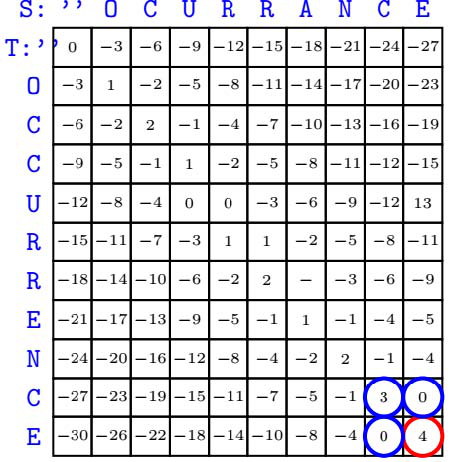
\includegraphics[width=2.4in]{alignment25.png}
\end{figure}

 第一行是说T是空时,是怎么一步步从$""$变化到 $S[1,..,n]$ 的。相当于每次都需要插入一个字母变成与S 对应的字母,即每增加一个字母就扣三分。

 第一列是说字典里有个词T,你敲成空字符串了,即表示T是怎么样变化到空字符串的,所以每次都少敲了,因此将T 变成S需要每次都删除一个字母,即每删除一个字母就扣三分。


\newpage

\subsection{构建最优解方案:}

那么我们如何知道最后的得分是怎么来的呢?常用的想法就是回溯,我们的最后的得分4本身有三个来源,我们开个表格记录该单元的得分是从三个来源中具体的哪个单元过来的,不断的向前回溯就可以找到一个对应的alignment,使得S变成T。

但是我们经常对分的评判不是很准确,这时候可以随机回溯多次,然后取平均,这样可以取一个比较常见的模式,使得我们最终得到的结果更稳定些。


现在对我们的问题再陈述下:我们在文档里面敲了一个词,该词不在词典中,这时候我们知道自己敲错了,但是我们想知道是怎么错的,我们想用这个分来衡量词典中的词经过最少的几次操作才能变成我们敲的单词S呢。

